\chapter{Diseño e implementación} % Main chapter title

\label{Chapter3} % Change X to a consecutive number; for referencing this chapter elsewhere, use \ref{ChapterX}





%----------------------------------------------------------------------------------------
%	SECTION 1
%----------------------------------------------------------------------------------------

\section{Propuesta de solución}

Este trabajo presenta una propuesta de solución a partir del desarrollo de un prototipo mínimo viable de un sistema IoT para integrar, centralizar y unificar resultados de una red de sensores y actuadores, mediante un sistema web de monitoreo y control, así como la construcción de módulos propios para dicha tarea, sin la necesidad de una conexión a Internet para su funcionamiento. 

Todos estos componentes trabajan en conjunto para brindar al cliente una solución tecnológica que sirva como herramienta visualmente amigable y que pueda ser el soporte en las tareas de gestión de consumo eléctrico. Para lograrlo, se desarrollaron módulos que integran \emph{software} y \emph{hardware}, estos hacen posible la adquisición de datos de sensores y actuadores ubicados en distintos puntos de una vivienda, conectados a una red local vía Wi-Fi. Cada lectura de los sensores permite el envío de datos a un servidor central local mediante el protocolo MQTT por vía inalámbrica, siendo el módulo principal local el responsable de registrar los valores de los sensores ante cualquier corte de Internet. La figura \ref{fig:diagrama1} ilustra el diagrama de componentes del sistema y la lógica de conexión.

\begin{figure}[htbp]
	\centering
	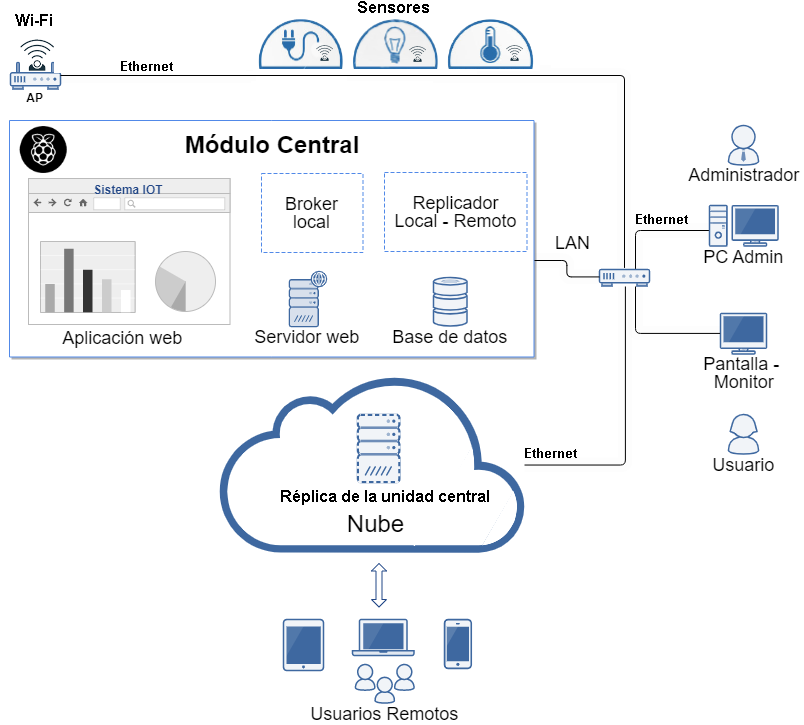
\includegraphics[width=0.92\textwidth]{./Figures/diagrama1.png}
	\caption{Diagrama de componentes del sistema.}

	\label{fig:diagrama1}
\end{figure}

El sistema tiene la capacidad de permitir el acceso por medio de cualquier dispositivo que cuente con un navegador web y con conectividad a Internet a cualquier usuario, ya sea desde dentro de la red local o desde fuera. Para alcanzar esta funcionalidad, fue necesario desarrollar un módulo \emph{software} que permita la replicación de datos desde la red local hacia un broker remoto ubicado en la nube. La necesidad de replicación de los datos hacia la nube solo se da mientras exista conexión a Internet. Para los casos de corte de Internet, el módulo replicador enviará los datos de forma automática la próxima vez que detecte el servicio de conexión a Internet. En la tabla \ref{tab:tablamodulos} se detalla el tipo de desarrollo para cada uno de los módulos del sistema  que se describe en las secciones siguientes.

\begin{table}[h]
	\centering
	\caption[Desarrollo integrado por módulo]{Desarrollo integrado por módulo}
	\begin{tabular}{l c c }    
		\toprule
		\textbf{Módulo} 	 & \textbf{Desarrollo}  & \textbf{Tipo dispositivo}\\
		\midrule
		Módulo principal & Hardware + Software & Físico\\		
		Módulo replicador & Software (procesos internos)& Lógico \\
		Módulo réplica & Software - remoto & Lógico \\
		Módulo de temperatura & Hardware + Firmware + Software & Físico\\		
		Módulo actuador & Hardware + Firmware + Software & Físico\\		
		Módulo de consumo	 & Hardware + Firmware + Software & Físico\\
		
		\bottomrule
		\hline
	\end{tabular}
	\label{tab:tablamodulos}
\end{table}


\section{Arquitectura IOT de la solución}

Existen tres componentes claves dentro de la solución propuesta y se mencionan en la arquitectura IoT diseñada durante el proceso de desarrollo: 


\begin{itemize}
\item Dispositivos IoT: son los módulos diseñados a partir de la integración de software, firmware y hardware; es posible conectarlos de forma inalámbrica a una red más amplia.
\item Redes: los routers domésticos, puntos de acceso y las configuraciones de las redes o las puertas de enlaces son los responsables de conectar varios dispositivos IoT a la nube.
\item Nube: servidores remotos en centros de datos que consolidan y almacenan la información con seguridad. Son servicios utilizados en el trabajo para garantizar el acceso remoto de usuarios al sistema.
\end{itemize}
\vspace{0.5cm}
Cada uno de estos componentes son adecuados para diferentes usos y va a depender de varios factores como, por ejemplo:

\begin{itemize}
\item Velocidad de transferencia de datos: ¿Cuánta información se enviará?
\item Consumo de energía: ¿Tienen una batería con una vida útil pequeña?, ¿Se puede usar con un trasformador conectado al servicio eléctrico?
\item Rango: ¿Necesita transmitir a unos pocos metros o a unos pocos kilómetros?
\item Frecuencia: ¿Cuáles son las frecuencias disponibles en la región?
\end{itemize}

\vspace{0.5cm}

Para este trabajo se realizó un análisis para cada interrogante dando como resultado el diseño de una arquitectura de integración funcional según los requerimientos  planteados al inicio. La figura \ref{fig:arquitectura} Ilustra la arquitectura resultado de la solución.

\section{Servicios en la nube}

Para el trabajo se consideró el servicio de \emph{cloud computing} tipo PaaS, porque permite la creación y configuración del broker remoto, el servidor Apache para la aplicación web y el gestor de base de datos MySQL.

El plan utilizado se divide en dos categorías, la primera está definida por el servicio del servidor web para alojar la aplicación web de monitoreo y control (réplica) y la segunda por el servicio del broker remoto que permite la comunicación directa con el broker local. 

La comunicación entre ambos servicios se hace mediante el protocolo MQTT utilizando la biblioteca  \emph{Eclipse Paho JavaScript Client}, se puede encontrar mayor información en la página oficial: \url{https://www.eclipse.org/paho/index.php} 

Las principales características  del servicio contratado para la implementación del prototipo mínimo viable se muestran en la tabla \ref{tab:serverweb}.


\begin{table}[h]
	\centering
	\caption[Características del servicio en la nube]{Características del servicio en la nube}
	\begin{tabular}{p{7cm} p{5cm} }    
		\toprule
		\textbf{Característica} 	 & \textbf{Detalle}  \\
		\midrule
		Sistema operativo  & GNU/Linux Centos\\		
		Espacio de almacenamiento & 1000 MB \\
		Transferencia mensual  & 10 GB\\		
		Multidominio & 2 dominios\\		
		Cantidad base de datos 	  & Ilimitados\\
		Subdominios 	  & Ilimitados\\
		Acceso FTP 	  & Si\\
		Backup diario y semanal 	  & Si\\
		Panel de control en español (CPanel) 	  & Si\\
		Soporte 24/7 	  & Si\\
		Seguridad - Firewall	  & Si\\
		Certificados SSL/TLS	  & Si\\
		PHP	  & V7 y V8\\
		MySQL	  & Si\\
		phpMyAdmin	  & Si\\
		PostgreSQL	  & Si\\
		phpPgadmin	  & Si\\
		Cron Jobs	  & Si\\
		\bottomrule
		\hline
	\end{tabular}
	\label{tab:serverweb}
\end{table}

\vspace{0.5cm}
%%%%%%%%%%%%%%%%%%%%%%%%%%% imagen horizontal%%%%%%%%%%%%%%%%%%%%%%%%%%%%%%%%%%%%%%%%%%%%
\begin{landscape} % esto es para rotar la pagina e imagen
\begin{figure}[htpb]
\centering 
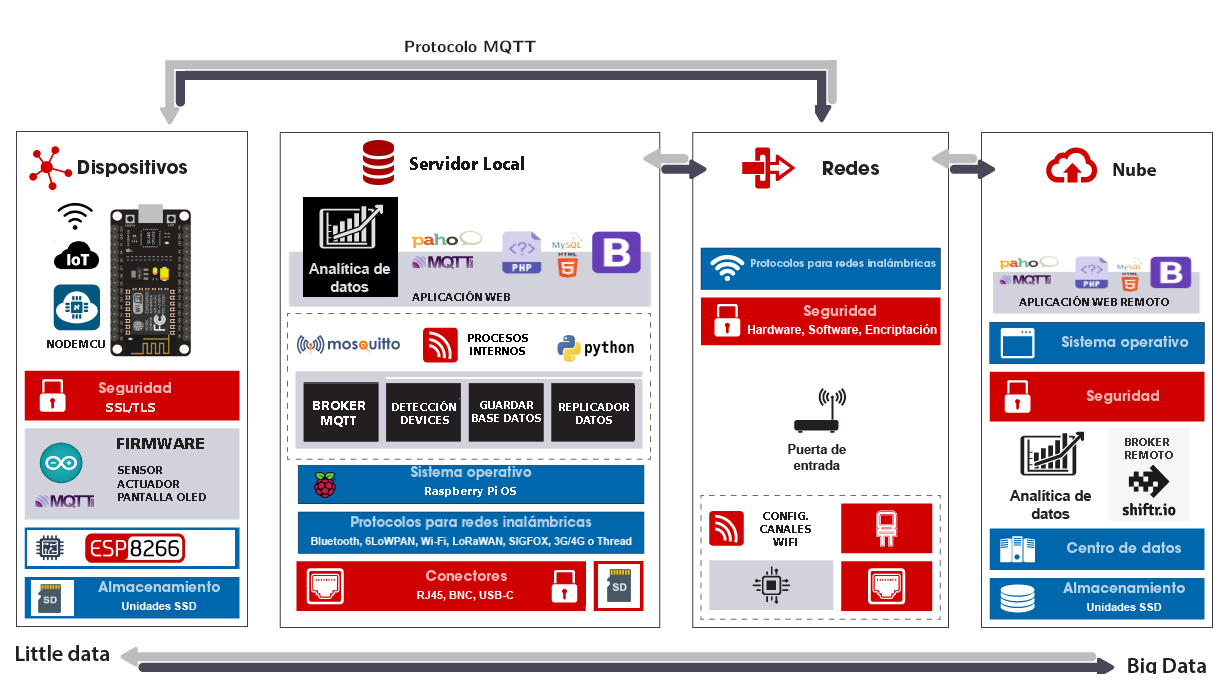
\includegraphics[width=1.65\textwidth]{./Figures/arquitectura-listo.png}
\caption{Arquitectura diseñada para el sistema IoT.}
\label{fig:arquitectura}
\end{figure}
\end{landscape} % esto es para rotar
%%%%%%%%%%%%%%%%%%%%%%%%%%%%%%%%%%%%%%%%%%%%%%%%%%%%%%%%%%%%%%%%%%%%%%%%%%

Las características del servicio para broker remoto se muestran en la tabla  \ref{tab:brokerremoto}

\begin{table}[h]
	\centering
	\caption[Características del broker remoto]{Características del broker remoto}
	\begin{tabular}{p{5cm} p{7cm} }    
		\toprule
		\textbf{Característica} 	 & \textbf{Detalle}  \\
		\midrule
		Conexiones activas  & 200\\		
		Mensajes por segundo & 10 k \\
		Interface  & MQTT Interface, HTTP interface\\		
		Compatibilidad & Arduino, JavaScript, Processing, Ruby \\		
		Deployment 	  & Por instancias\\
		Envíos y recepción de datos & objetos codificados JSON\\
		
		\bottomrule
		\hline
	\end{tabular}
	\label{tab:brokerremoto}
\end{table}

\section{Medidas de ciberseguridad}

Los requerimientos de ciberseguridad dentro del desarrollo ocupan un lugar muy importante en cada una de las etapas ejecutadas en el proceso de implementación de un sistema IoT, porque permite garantizar un grado mínimo de seguridad y confiabilidad funcional del producto. 

Los requerimientos considerados durante el proceso, son los siguientes:

\subsection{Requerimientos para la aplicación de monitoreo y control}

\begin{itemize}
\item Encriptación de claves de acceso, la longitud de cadena de las claves  deben ser mayor a 8 dígitos, considerando números, letras mayúsculas, letras minúsculas, números y símbolos especiales.
\item Medidas de protección contra \emph{Injeccion SQL} y usar sentencias preparadas u objetos PDO (\emph{PHP Data Objects}) para las conexiones hacia la base de datos.
\item Control de acceso por CORS (\emph{Cross Origin Resource Sharing}) para recursos de la API REST.
\item Configuración del archivo .htaccess para evitar listado de directorios o accesos no permitidos.
\item Minificar los archivos CSS (\emph{Cascading Style Sheets}) y JS (\emph{JavaScript}) de la aplicación web.
\item Control de acceso al sistema según validación de roles y permisos.
\item Uso de la programación orientados a objetos.
\item Uso de peticiones POST como prioridad, si fuera necesario el uso de las peticiones GET, utilizarlas con el paso de parámetros encriptados.
\end{itemize}

\subsection{Requerimientos para el broker local y remoto}

\begin{itemize}
\item Configuración de usuario y contraseña para controlar el acceso a los canales de comunicación del broker local y remoto.
\item Uso de canales separados, para el envió, sincronización y respuesta entre elementos del sistema IoT.
\item Cada mensaje debe ir con destino a un tópico en específico, evitar envió de datos a la instancia general \#.
\item Configurar permisos para la edición o ejecución a los archivos de configuración del broker.
\end{itemize}

\subsection{Requerimientos para los módulos IoT}

\begin{itemize}
\item Uso de programación basada en código modular para el desarrollo del firmware.
\item Uso de la biblioteca en su versión más actual para la comunicación MQTT.
\item Los objetos de datos a transmitir serán del formato JSON.
\item La comunicación el protocolo MQTT debe contener TLS.
\end{itemize}

\subsection{Requerimientos para la red WLAN}

\begin{itemize}
\item Uso de un AP (\emph{Access Point}) como elemento central para el servicio Wi-Fi independiente (dedicado solo para el sistema IoT) para garantizar una subred paralela al usado para la red doméstica.
\item Configuración ideal del canal de comunicación inalámbrica, para evitar el uso de un canal con alto grado de solapamiento.
\item Uso de dispositivos AP con la función de seguridad de clave WPA2-PSK (AES).
\item Configurar el nombre de la señal por defecto, la clave de acceso al AP y a la señal Wi-Fi, considerando letras minúsculas, mayúsculas, números y símbolos especiales.
\item Monitoreo continuo de la red Wi-Fi del AP, para supervisar la presencia únicamente de solo dispositivos válidos en la red dedicada.
\end{itemize}


\subsection{Requerimientos para el servidor local}

\begin{itemize}
\item Sistema operativo GNU/Linux oficial Raspberry Pi OS.
\item Acceso al sistema operativo mediante usuario y contraseña.
\item Accesos remotos por SSH (Secure Shell) y FTP (File Transfer Protocol)  desactivados.
\item Cifrado de las unidades del sistema operativo.
\end{itemize}

\section{Diseño e implementación de módulos}

En esta sección se describen el proceso y consideraciones técnicas para la construcción de cada uno de los módulos del sistema IoT propuesto.

\subsection{Módulo principal (servidor local)}

El modulo principal representa el elemento central dentro de la solución IoT planteada. Para la construcción e instalación se utilizaron recursos que hicieron posible lograr una versión de fácil uso para el usuario.

Está conformado por una placa Raspberry Pi 4 modelo B con 8 GB de memoria RAM, su fuente de alimentación de 3 A como se aprecia en la figura \ref{fig:placarpi4}.

La unidad de almacenamiento contiene una unidad de memoria extraíble microSD de 64 GB y de clase 10 para garantizar alta velocidad de lectura y escritura durante el procesamiento.
% La figura \ref{fig:microsd} muestra la microSD del módulo.

\begin{figure}[htpb]
\centering 
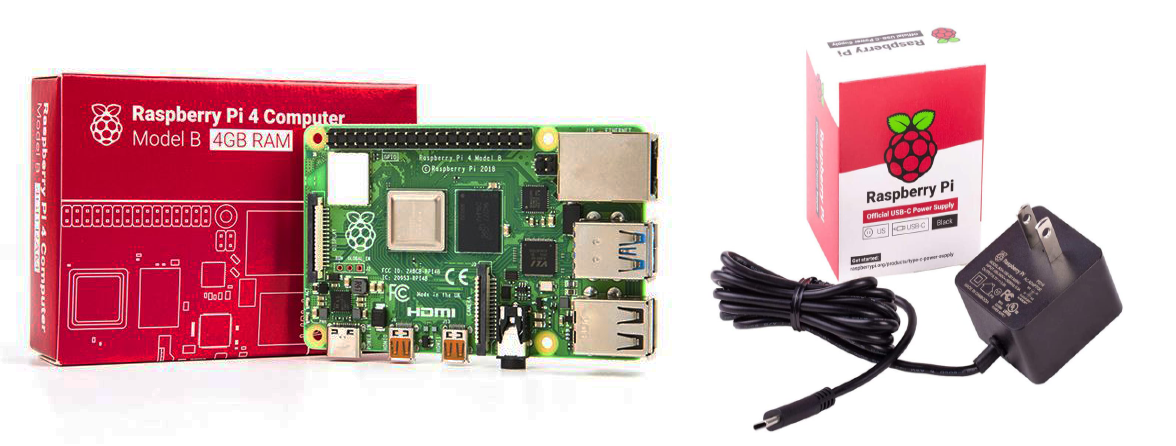
\includegraphics[width=0.9\textwidth]{./Figures/placa.png}
\caption{Mainboard y fuente de alimentación del servidor local.}
\label{fig:placarpi4}
\end{figure}
%\begin{figure}[htpb]
%\centering 
%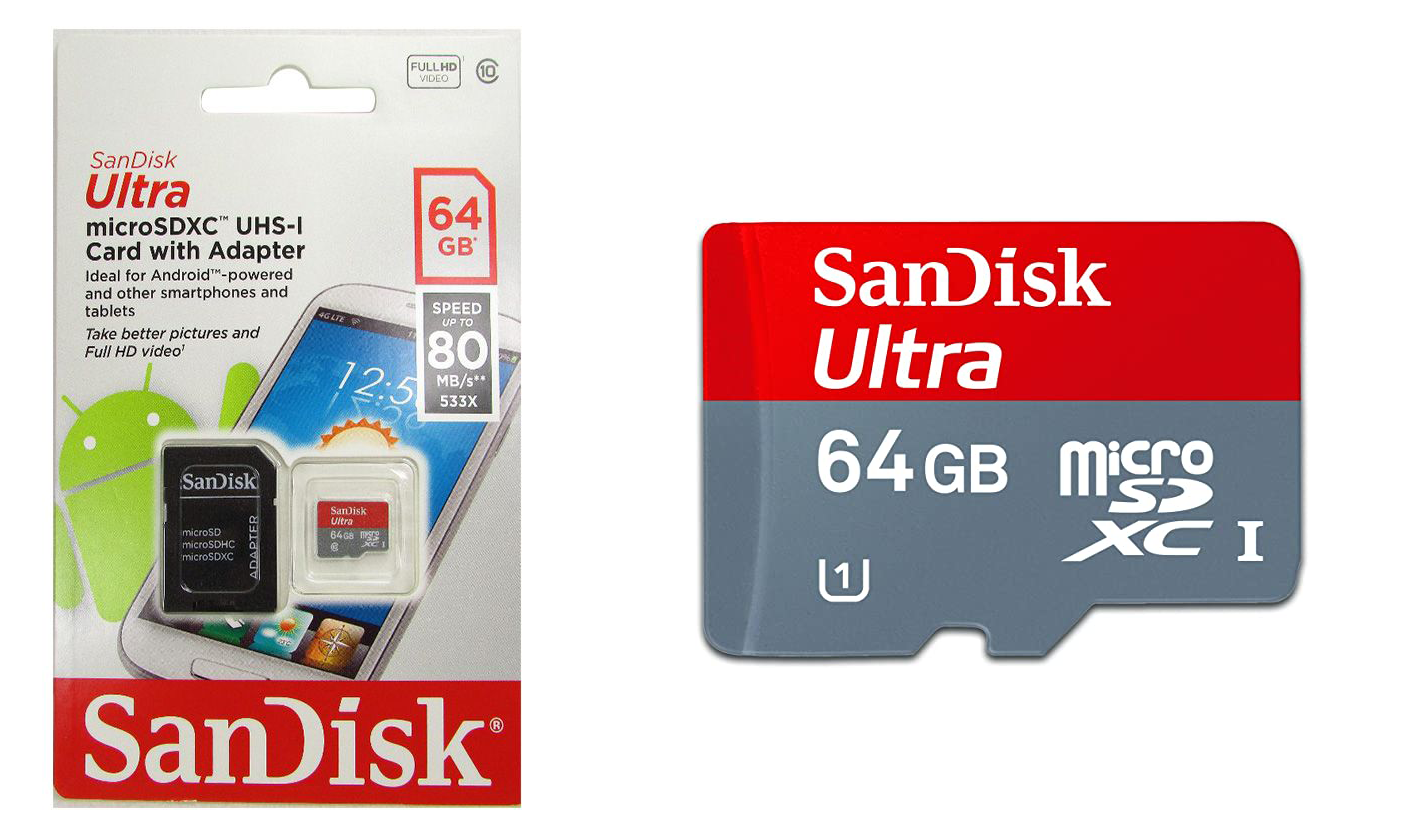
\includegraphics[width=0.7\textwidth]{./Figures/card.png}
%\caption{Tarjeta de almacenamiento del servidor local.}
%\label{fig:microsd}
%\end{figure}
Para el gabinete de integración se consideró una cubierta de aluminio. La figura \ref{fig:armado} muestra el ensamblado de la placa y el case Argon One Pi4 V2 del módulo principal.

\begin{figure}[htpb]
\centering 
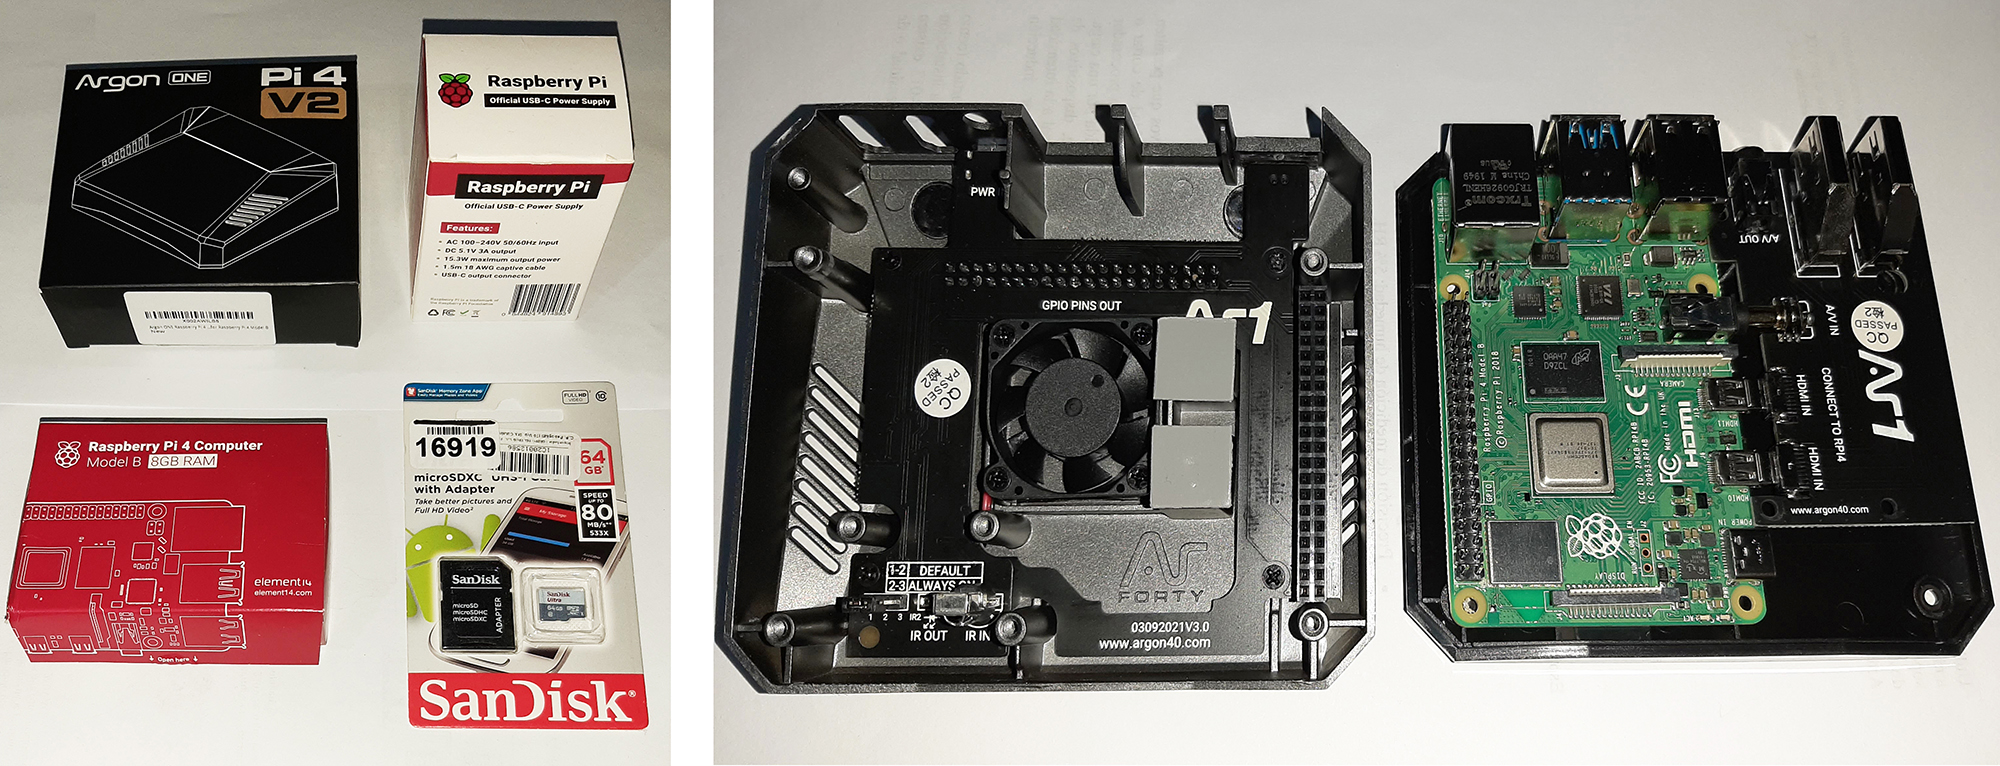
\includegraphics[width=1.0\textwidth]{./Figures/m1-2.jpg}
\caption{Componentes y ensamblado del módulo principal.}
\label{fig:armado}
\end{figure}

\vspace{0.5cm}
Características del case de integración Argon One Pi4 V2 \citep{WEBSITE:16}:

\begin{itemize}
\item Tiene una placa Raspberry Pi Sata, que está diseñada para maximizar las transferencias de datos de alta velocidad para el uso de SSD Raspberry Pi 4; lo que la hace perfecta para el uso multimedia y otras aplicaciones. 
\item La funda SSD Raspberry Pi solo es compatible con SSD M.2 SATA con llave B-Key o B+M.
\item El SSD se conecta al Raspberry Pi 4 a través del puente USB en un puerto USB 3.0. 
\item El case Argon incluye dos puertos HDMI de tamaño completo e IR integrado para la funcionalidad remota y también posee arranque automático. 
\item El case Argon Raspberry Pi 4 tiene todos los pines GPIO accesibles en la parte superior de la funda mientras están protegidos por una cubierta magnética extraíble cuando no están en uso. 
\item El case Argon ONE Raspberry Pi 4 obtiene la mejor experiencia de refrigeración gracias al \emph{software} Pi Fan mientras que la funda actúa como un disipador de calor conectado a la CPU.
\end{itemize}

El modulo principal tiene la capacidad de conectarse a la red vía Wi-Fi o vía Ethernet. La integración y partes del módulo se muestra en la figura \ref{fig:argon}.



%%%%%%%%%%%%%%%%%%%%%%%%%%% imagen horizontal%%%%%%%%%%%%%%%%%%%%%%%%%%%%%%%%%%%%%%%%%%%%
%\begin{landscape} % esto es para rotar la pagina e imagen
\begin{figure}[htpb]
\centering 
%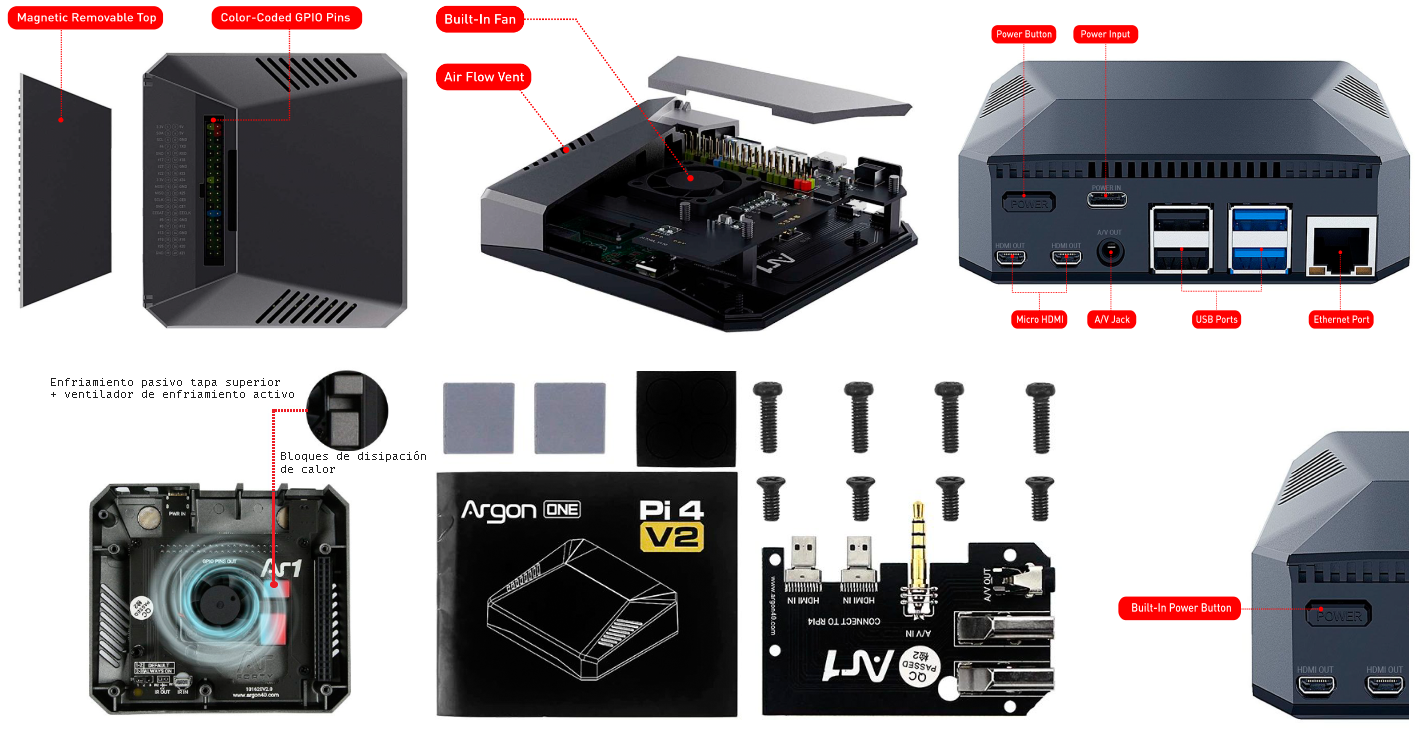
\includegraphics[width=1.7\textwidth]{./Figures/argon.png}
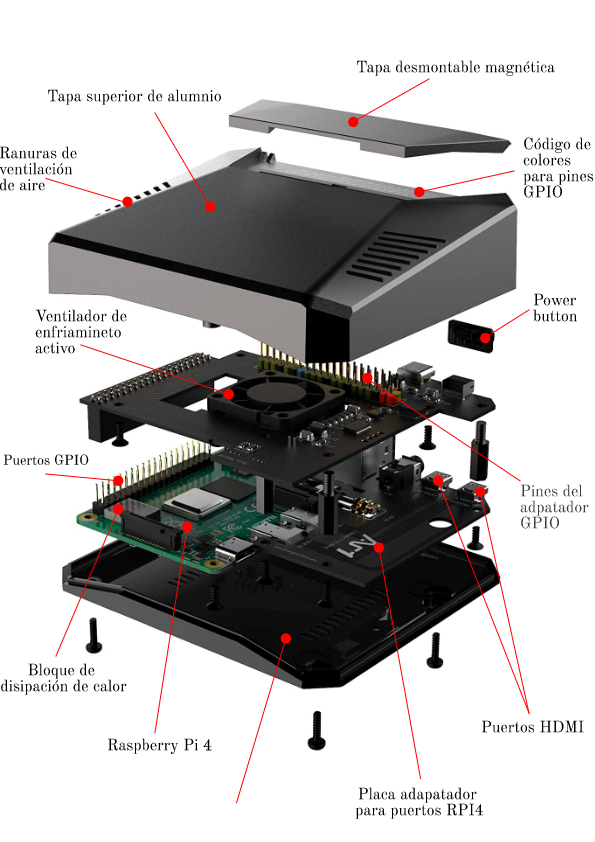
\includegraphics[width=0.94\textwidth]{./Figures/armadoactuador.png}
\caption{Ensamblado y partes del módulo principal. }
\label{fig:argon}
\end{figure}
%\end{landscape} % esto es para rotar
%%%%%%%%%%%%%%%%%%%%%%%%%%%%%%%%%%%%%%%%%%%%%%%%%%%%%%%%%%%%%%%%%%%%%%%%%%%


\subsection{Módulo replicador a la nube}

Este módulo esta dentro del módulo principal y para su desarrollo de se diseñó una estructura interna compuesta por subprocesos, que al trabajar en conjunto forman el sistema completo de replicación.

La replicación solo se da mientras exista conexión a internet. El desarrollo de cada subproceso se programó en el lenguaje de programación Python por tratarse de un lenguaje multiplataforma, robusto y orientado a objetos. La figura \ref{fig:logicareplicador} ilustra la lógica de trabajo del replicador.


%\begin{figure}[htpb]
%\centering 
%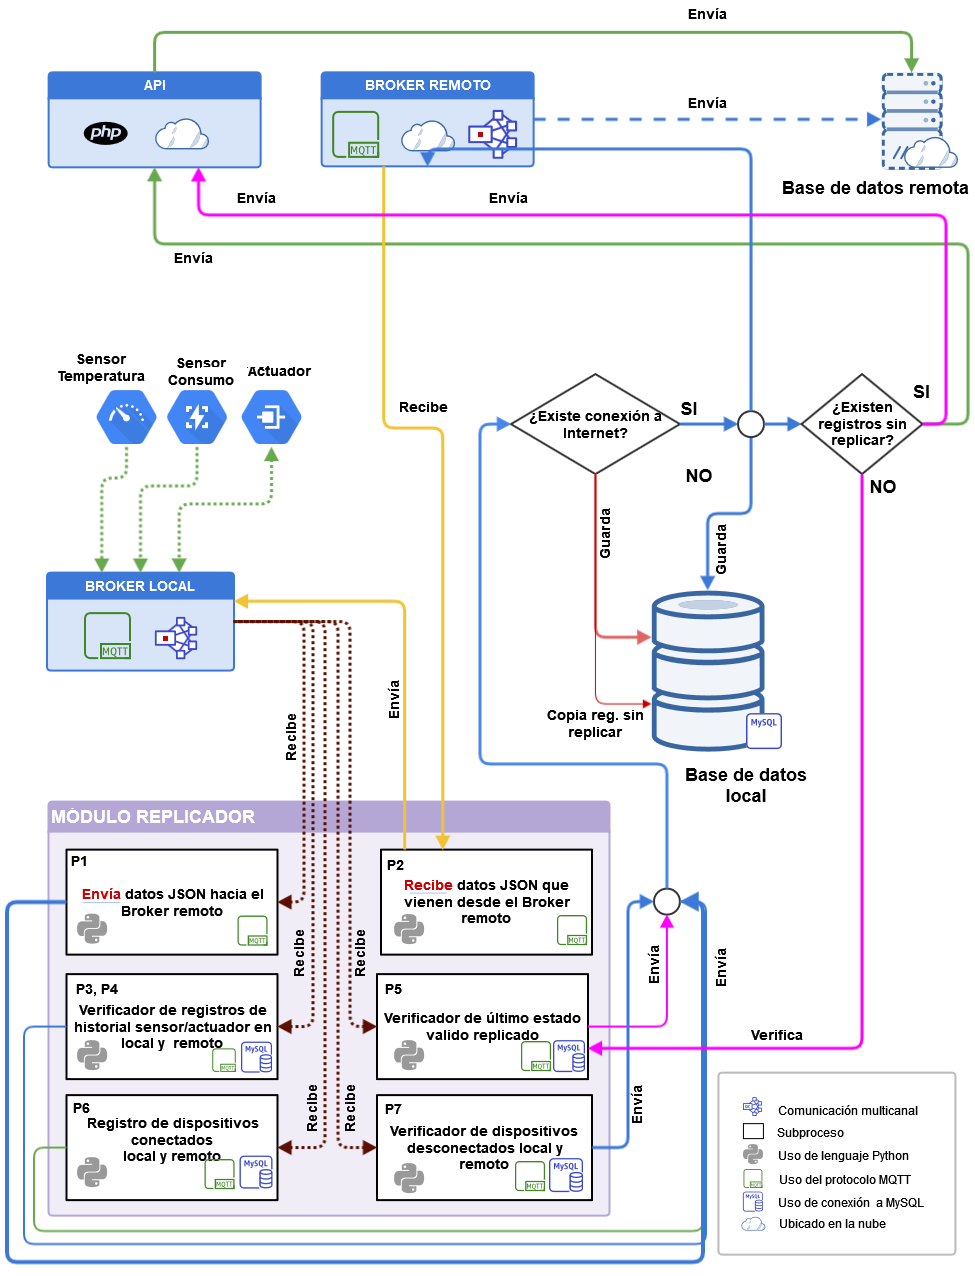
\includegraphics[width=1.15\textwidth]{./Figures/replicador.png}
%\caption{Flujo funcional del módulo replicador.}
%\label{fig:flujoreplicador}
%\end{figure}



Las descripciones de cada subproceso interno que contiene el módulo replicador, se detallan a continuación: 

\begin{itemize}
\item \keyword{mqtt\_envia\_nube\_poo (P1)}: es el responsable de enviar todos los datos que llegan de los canales hacia el broker remoto usando el formato JSON.

\item \keyword{mqtt\_recibe\_nube\_poo (P2)}: es el responsable de recibir los datos JSON que fueron generados en la aplicación web remota y que llegan desde el broker remoto para luego transmitirlo.

\item \keyword{actuador\_registros\_bd (P3)}: es el responsable de verificar los registros en la base de datos. Su verificación está basada en intervalos de tiempo de una hora, consulta todos los registros de lecturas de actuadores capturadas dentro de una hora en las tablas auxiliares de actuadores y consumos para luego sumar el consumo y hacer un solo registro en la tabla de historial de consumo. Este subproceso realiza un borrado de registros de las tablas auxiliares de actuadores por cada registro en la tabla historial.

\item \keyword{sensor\_registros\_bd (P4)}: es el responsable de verificar los registros en la base de datos. Su verificación está basada en intervalos de tiempo de una hora, consulta todos los registros de lecturas de sensores capturadas dentro de una hora en las tablas auxiliares de sensores, para luego promediarlos y hacer un solo registro en la tabla de historial. Este subproceso realiza un borrado de registros de las tablas auxiliares de sensores por cada registro en la tabla historial.

\item \keyword{sensor\_historial\_replicas\_bd (P5)}: es el responsable de verificar de forma constante la conexión a Internet y si existen datos por replicar, en caso de disponer de una conexion a Internet y a partir de registros marcados como no replicados, este procederá a enviar los últimos registros hacia la nube, para luego limpiar la tabla de registros\_no\_enviados, y así mantener la consistencia necesaria para el sistema local y remoto.

\item \keyword{mqtt\_gestionBD\_poo (P6)}: es el responsable de recibir todos los mensajes que llegan al broker y verificar la pertenencia del JSON capturado (sensor o actuador) para, posteriormente comprobar si existe conexión a Internet y poder registrar en la base de datos local y remoto. En caso que no existiera conexión a Internet, solo registra en la tabla correspondiente al sensor o actuador de la base de datos local y a su vez realiza una copia hacia la tabla de registros\_no\_enviados, para que pueda ser enviado a la nube cuando vuelva a existir la conexión a Internet. Este subproceso también permite actualizar el estado de un sensor o actuador en la base de datos con el estado de ``CONECTADO'' mientras esté activo en la red.

\item \keyword{mqtt\_gestionDispositivosConectados (P7)}: es el responsable de recibir todos los mensajes que llegan al broker, verificar la pertenencia del JSON capturado (sensor o actuador) para registrar temporalmente el tiempo de llegada del mensaje del dispositivo. 

Este subproceso usa hilos en Python para estar constantemente registrando los tiempos de llegada de mensajes de cada sensor o actuador, y si los intervalos de tiempo de llegada de mensajes para un dispositivo activo son mayores a un minuto, el subpoceso actualiza el estado del dispositivo con el estado de ``DESCONECTADO'' en la base de datos.
\end{itemize}
%\vspace{0.05cm}
%%%%%%%%%%%%%%%%%%%%%%%%%%% imagen horizontal%%%%%%%%%%%%%%%%%%%%%%%%%%%%%%%%%%%%%%%%%%%%
%\begin{landscape} % esto es para rotar la pagina e imagen
\begin{figure}[htbp]
	\centering
	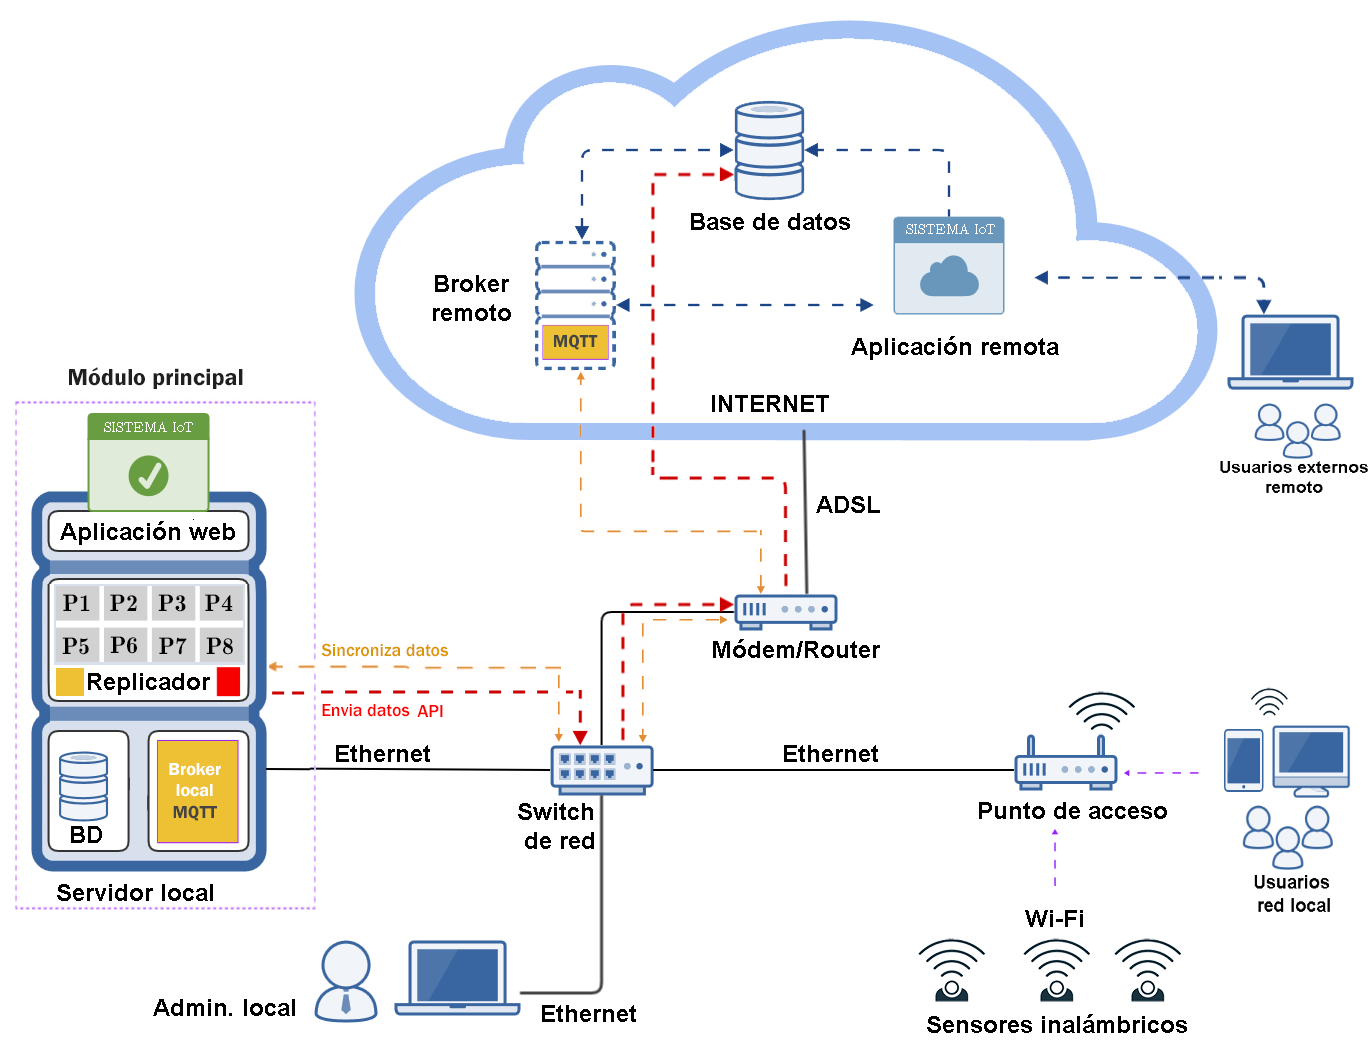
\includegraphics[width=1.0\textwidth]{./Figures/diagrama2.png}
	\caption{Diagrama funcional del replicador. }

	\label{fig:logicareplicador}
\end{figure}
%\end{landscape} % esto es para rotar
%%%%%%%%%%%%%%%%%%%%%%%%%%%%%%%%%%%%%%%%%%%%%%%%%%%%%%%%%%%%%%%%%%%%%%%%%%%

\subsection{Módulo de medición de temperatura}

Este módulo permite recoger lecturas del valor de la temperatura y humedad en ambientes de un hogar, oficina o edificio. Los valores son enviados y procesados en el sistema IoT de control y monitoreo que se encuentra en el servidor web del módulo principal. Las lecturas de temperatura son utilizadas para conocer la curva de cambios de temperatura según el horario registrado, así como su relación directa con el consumo eléctrico por el uso de ventiladores y equipos de aire acondicionado. Para su construcción se usó la placa NodeMCU8266 V3, por las características tales como: capacidad de conexión inalámbrica, bajo costo y tamaño reducido. 

Este módulo integra una pantalla SSD1306 OLED para visualizar el valor de la temperatura en tiempo real. Para el encapsulado y construcción se utilizó un tablero adosable de montaje de interruptores térmicos y diferenciales tipo RIEL-DIN, de material de poliestireno y cubierta trasparente de policarbonato con apertura vertical \citep{WEBSITE:17}, como se aprecia en la figura \ref{fig:casetemp}.


\begin{figure}[htpb]
\centering 
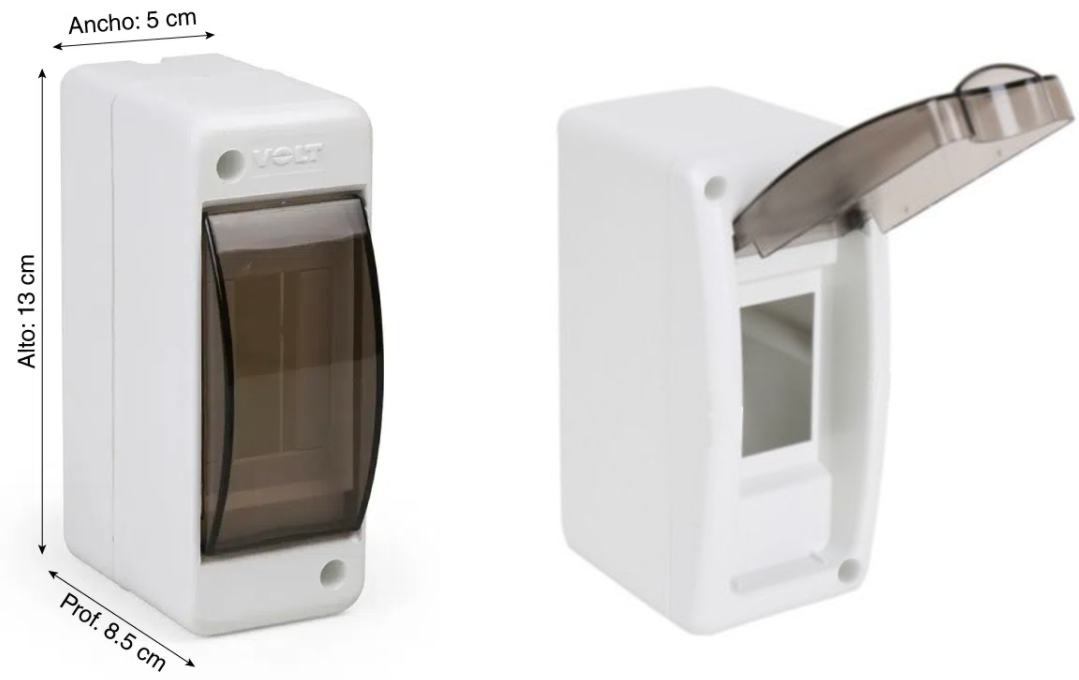
\includegraphics[width=0.7\textwidth]{./Figures/casetemp.png}
\caption{Case del módulo de temperatura \protect\footnotemark.}
\label{fig:casetemp}
\end{figure}

\footnotetext{Imagen tomada de \url{https://www.promart.pe/tablero-2-polos-adosable-c-puerta/p}}

El diseño de integración de componentes electrónicos se realizó en una Placa PCB perforada siguiendo el esquemático de la figura \ref{fig:citemp}.

\begin{figure}[htpb]
\centering 
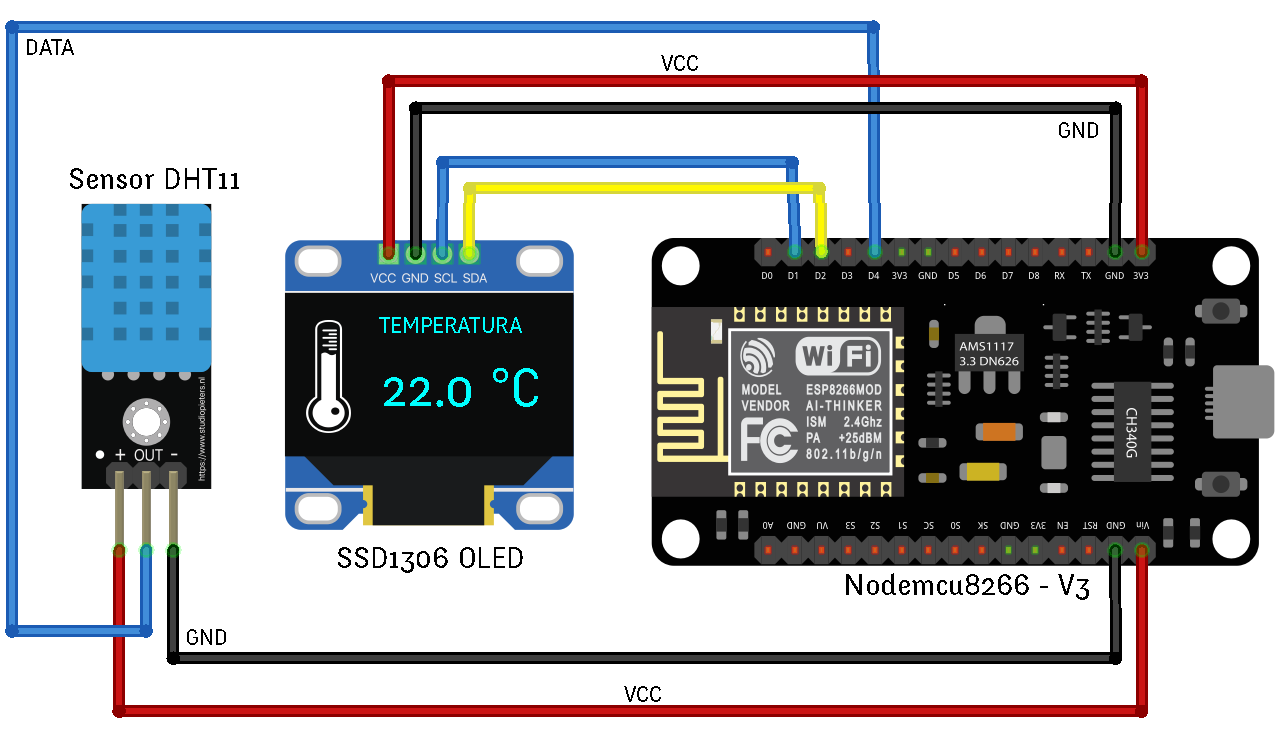
\includegraphics[width=1.0\textwidth]{./Figures/ci-temp.png}
\caption{Esquemático electrónico del módulo de temperatura. }
\label{fig:citemp}
\end{figure}

El proceso de integración total lo podemos ver en las fotografías que se visualizan en la figura \ref{fig:entemp}.

\begin{figure}[htpb]
\centering 
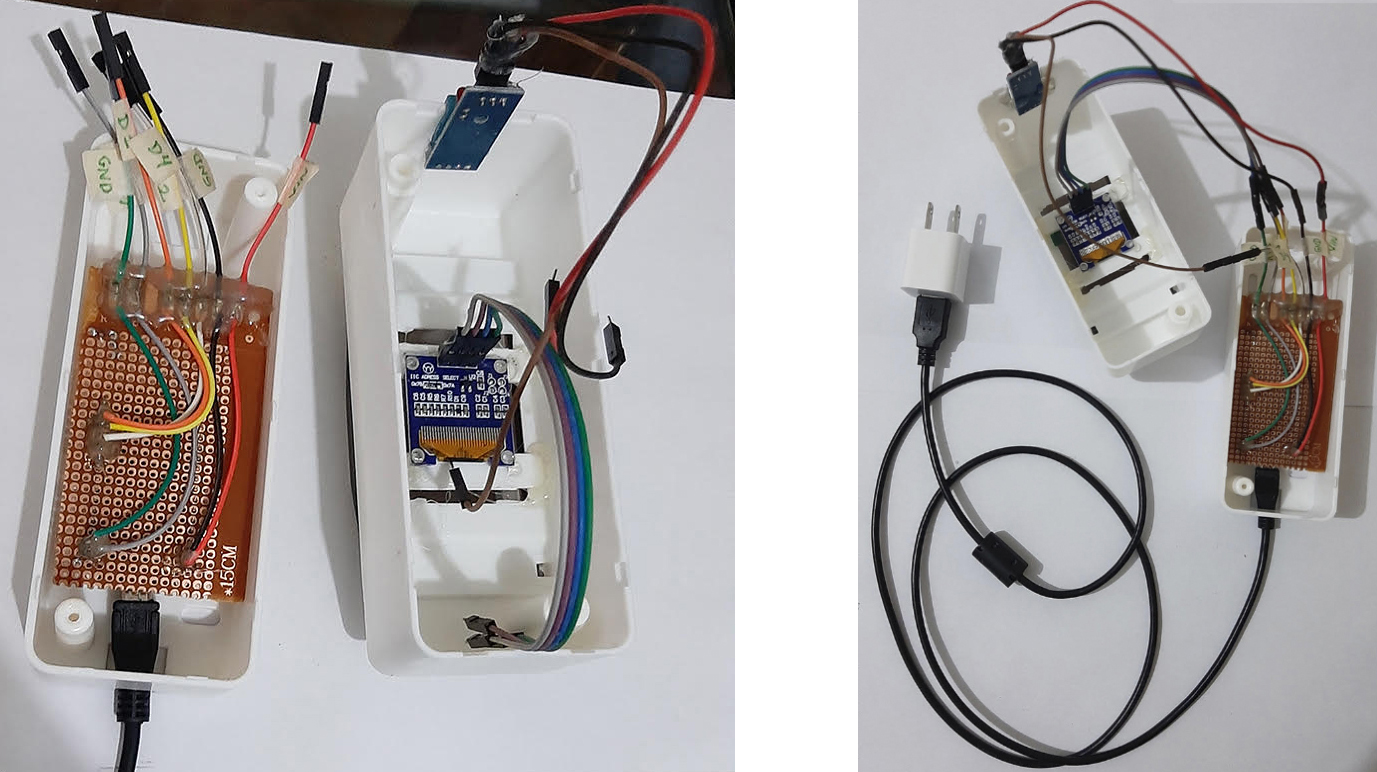
\includegraphics[width=0.95\textwidth]{./Figures/temperatura.jpg}
\caption{Ensamblado del módulo de temperatura. }
\label{fig:entemp}
\end{figure}

\subsection{Módulo actuador}

Este módulo permite activar o desactivar el paso de la corriente eléctrica dentro de un tomacorriente. La acción de cambio de estados (activado o desactivado) se realiza desde un switch en la interfaz de la aplicación web de monitoreo y control.

Para la construcción del módulo se utilizó una caja (case) de tomacorriente  resistente a impactos, de gran durabilidad, autoextinguible e Ideal para conductos de cables \citep{WEBSITE:18}, categoría 12 y 14. Para fijar el tomacorriente se usó una placa modular de soporte. En figura \ref{fig:caseactuador} se ilustran los componentes mencionados.

\begin{figure}[htpb]
\centering 
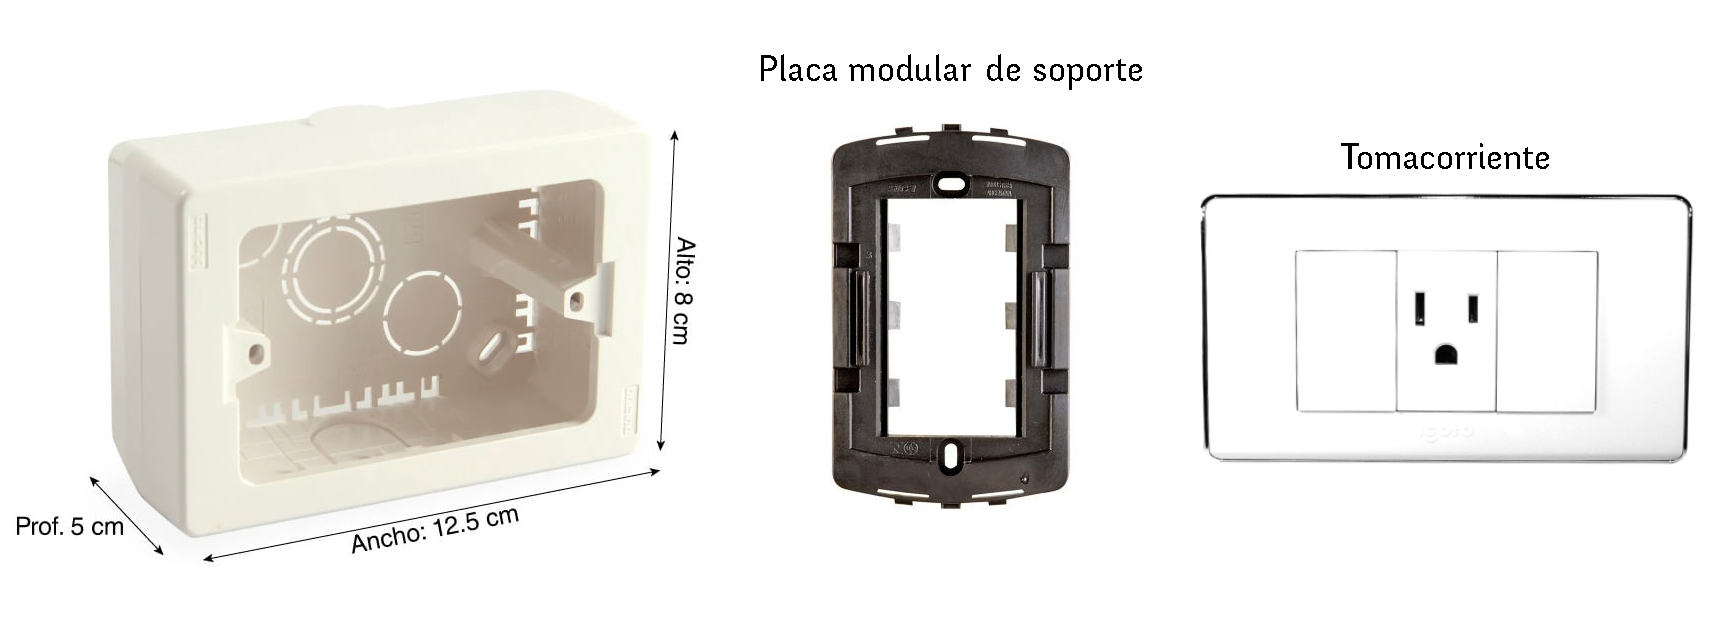
\includegraphics[width=1.0\textwidth]{./Figures/actuador.jpg}
\caption{Case del módulo actuador.}
\label{fig:caseactuador}
\end{figure}

Para la activación del relé de 5 V mediante una salida de la placa NodeMCU8266 fue necesario usar un convertidor de tensión DC-DC Step-Up 2 A MT3608, porque las salidas de la placa NodeMCU8266 son de 3.3 V y la activación del relé requiere 5 V para funcionar. El DC-DC Step-Up tiene como función entregar un tensión de salida constante superior a la tensión de entrada frente a variaciones a la tensión de entrada, soporta como tensión de entrada entre 2 V a 24 V y tensión de salida entre 2 V a 28 V. La tensión de salida se puede regular mediante un potenciómetro multivuelta \citep{WEBSITE:19}. La figura \ref{fig:esquemaactuador} ilustra el relé de 30 A y el convertidor de tensión utilizado para la solución a este problema.

\begin{figure}[htpb]
\centering 
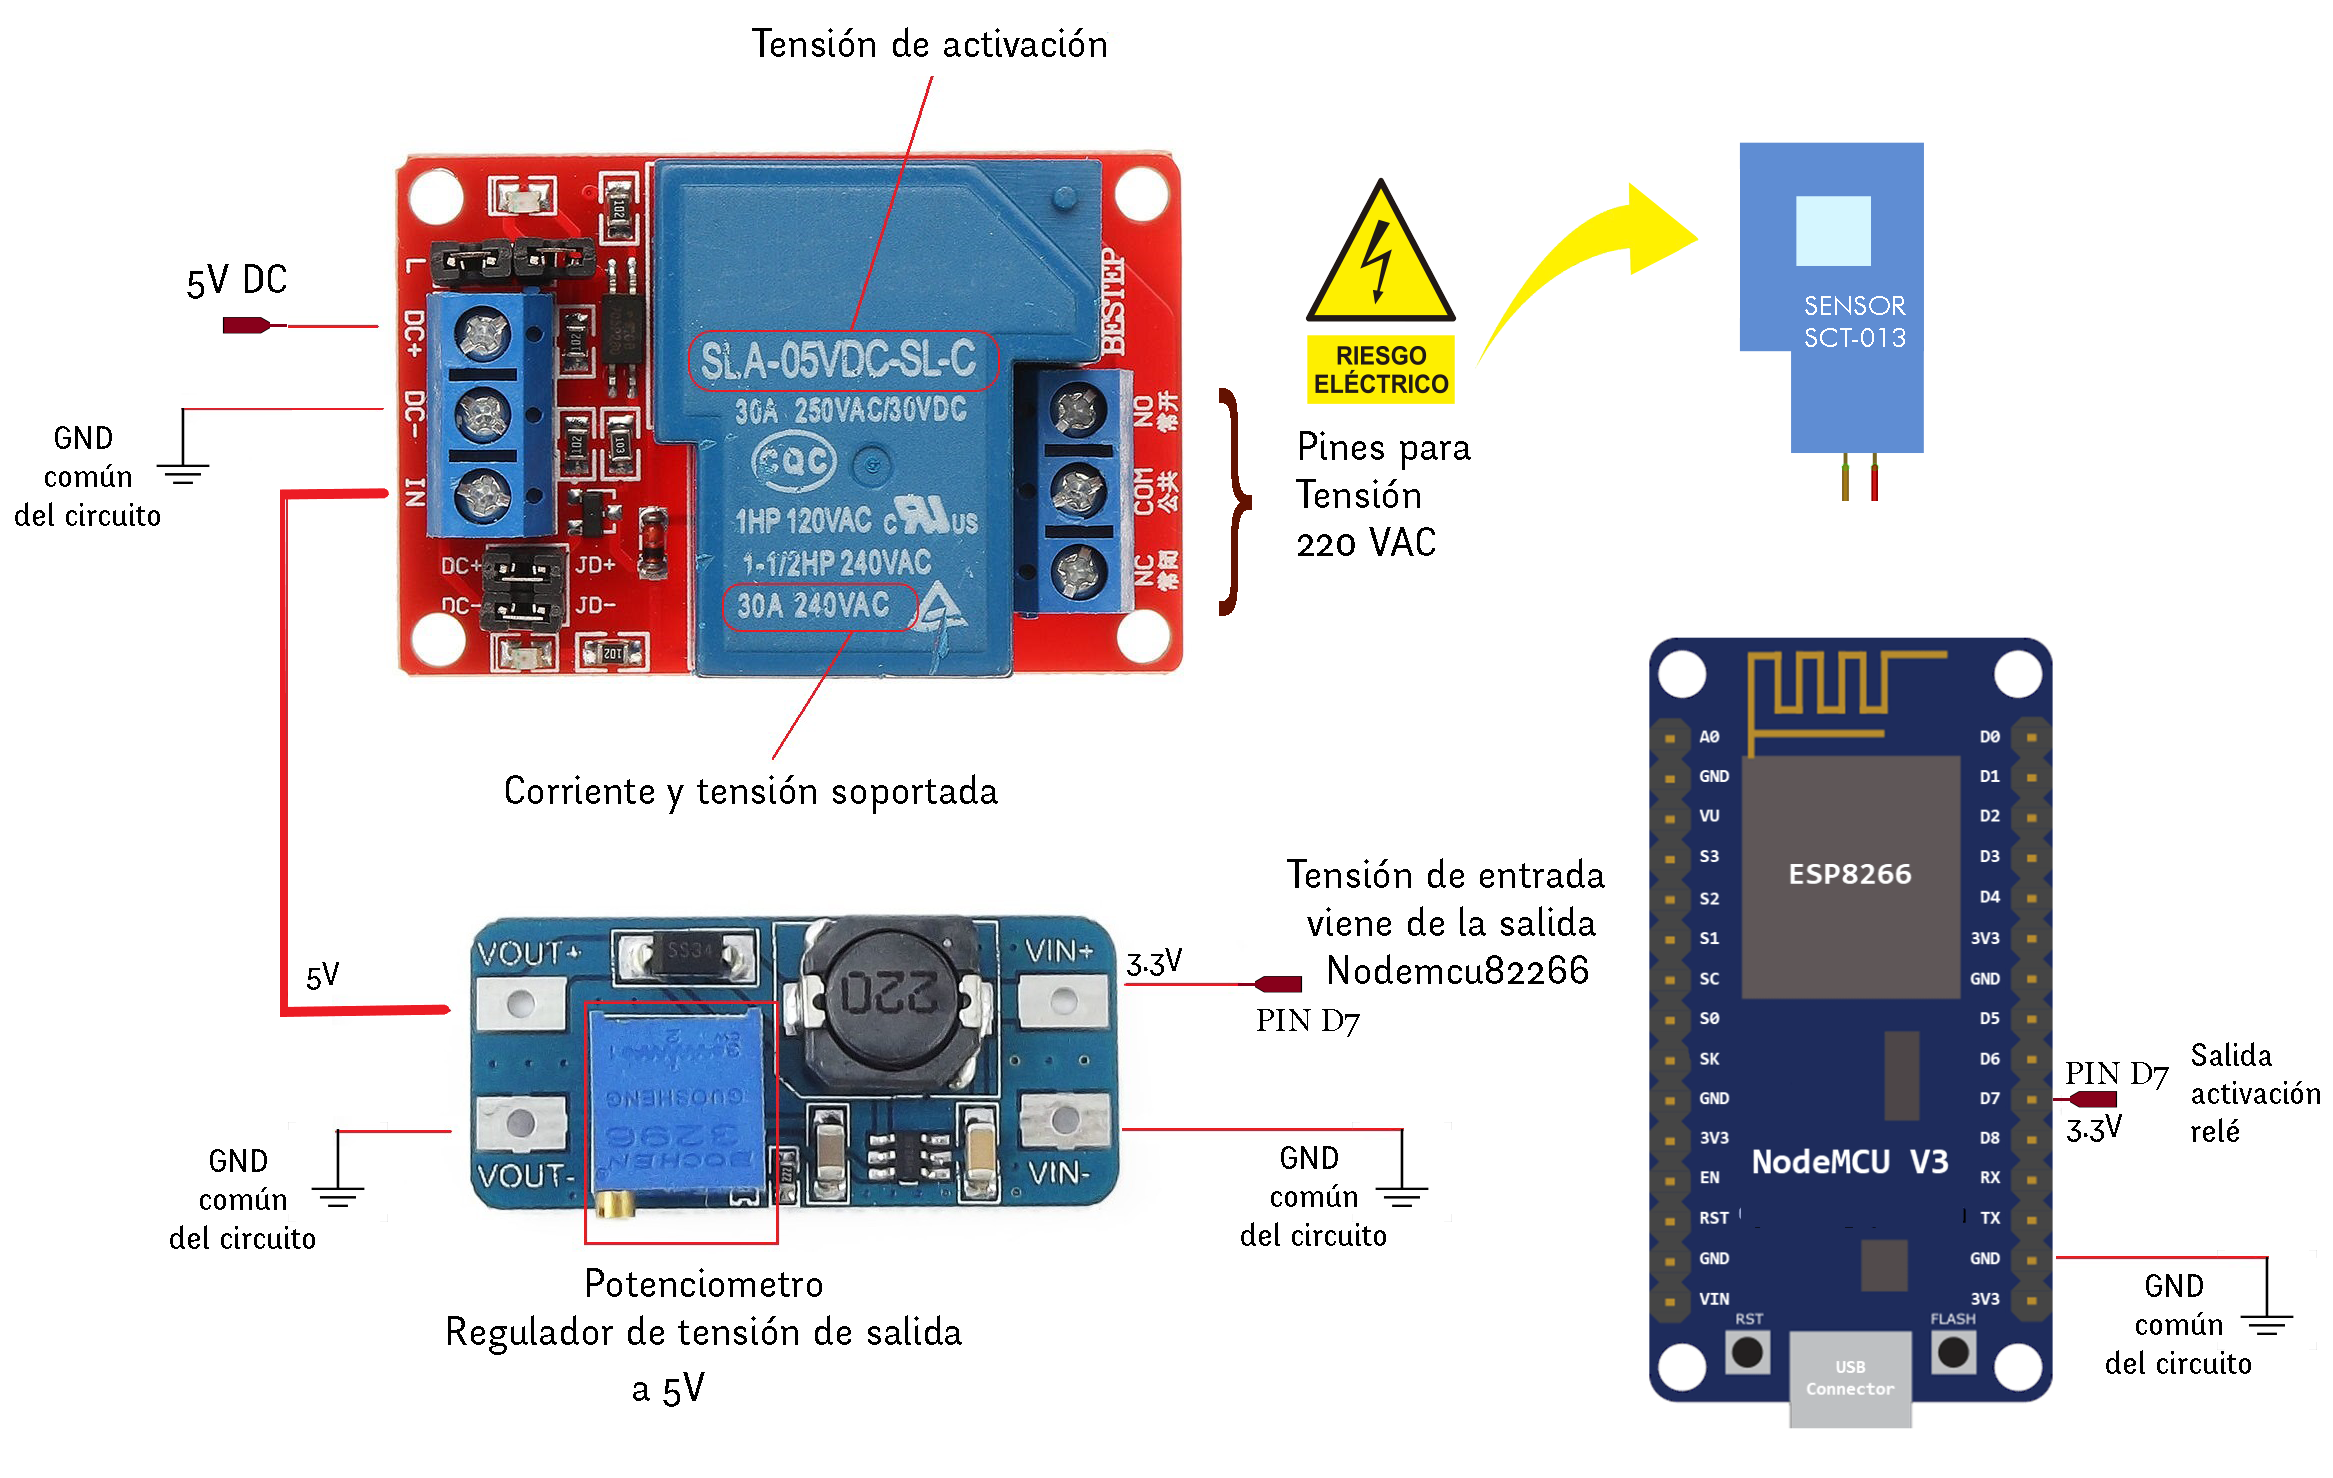
\includegraphics[width=1.057\textwidth]{./Figures/esquemaactuador.png}
\caption{Uso del Step-Up DC-DC para activación del relé. }
\label{fig:esquemaactuador}
\end{figure}

%\vspace{1cm}
%\vspace{1cm}

\subsection{Módulo de consumo eléctrico}

Este módulo es el responsable de medir el consumo de energía eléctrica dentro de un hogar, oficina o edificio. La integración de los componentes representó un gran reto dentro del proceso de construcción y desarrollo por ser un módulo que permite comunicación bidireccional con el servidor local y a su vez tener sincronización con todos los clientes conectados al sistema.

%\vspace{2cm}

\keyword{¿Cómo se mide el consumo de energía eléctrica?}

La energía eléctrica que consume un artefacto eléctrico, se determina multiplicando la potencia de dicho artefacto por la cantidad de horas que está encendido \citep{BOOK:3}. Por ejemplo ver la ecuación \ref{eq:consumoform}.

\begin{equation}
	\label{eq:consumoform}
	EC = \left( T x PE \right)
\end{equation}

\vspace{0.1cm}
Siendo las variables y unidades:
\begin{itemize}
\item EC: energía consumida (kWh)
\item T: tiempo que esta encendido (h)
\item PE: potencia eléctrica del artefacto (kW)
\end{itemize}

\vspace{0.1cm}
\keyword{¿Cómo se calcula la potencia eléctrica?}

El cálculo de la potencia eléctrica se obtiene al tener en cuenta la carga eléctrica, también conocida como tensión eléctrica, que pasa en un tiempo limitado a través de una diferencia de potencia, denominada intensidad. El resultado, cuya unidad es el vatio (en inglés, watt) su símbolo es la W , se obtiene al multiplicar la tensión por la intensidad. La tensión se pone en Voltios (V) y la Intensidad en amperios (A). La fórmula de la potencia eléctrica se ilustra en la ecuación \ref{eq:potenciaform} \citep{WEBSITE:20}.

\begin{equation}
	\label{eq:potenciaform}
	PE = \left( TE x IE \right)
\end{equation}

\vspace{0.2cm}
Siendo las variables y unidades:
\begin{itemize}
\item TE: tension eléctrica(V)
\item IE: intensidad eléctrica (A)
\item PE: potencia eléctrica del artefacto (W)
\end{itemize}


Como se observa en la ecuación \ref{eq:potenciaform}, para poder medir el consumo eléctrico se necesita medir la tensión (V) y la intensidad (A) eléctrica y para dicha tarea se utilizaron dos sensores, el sensor SCT-013-030 para medir intensidad de corriente alterna y el sensor AC - ZMPT101B para medir tensión eléctrica alterna.

Los aspectos más importantes para el diseño, desarrollo y construcción del módulo se describen  a continuación, así como conceptos técnicos específicos necesario para la programación del firmware y el proceso que permite almacenar los consumos electrónicos en la base de datos.


\begin{enumerate}
\item \keyword{Componentes para la construcción del módulo}
\begin{itemize}
\item Case de protección
\item Sensor de tensión eléctrica AC - ZMPT101B
\item Sensor de corriente eléctrica SCT-013-030
\item Convertidor ADC ADS1115
\item Cable de calibre 14:
\item Fusible de 30 A
\item Pantalla gráfica LCD
\item Fuente embebida input 220 V, output 5 V
\item Leds ultra brillantes:
\end{itemize}

\item \keyword{Aplicación del sensor SCT-013-030}

La familia SCT-013 son sensores de corrientes no invasivos que permiten medir la intensidad de corriente que atraviesa un conductor sin necesidad de cortar o modificar el conductor. Es posible emplear estos sensores con un procesador Arduino o derivados para medir la intensidad o potencia consumida por una carga. Los sensores SCT-013 son transformadores de corriente, dispositivos de instrumentación que proporcionan una medición proporcional a la intensidad que atraviesa un circuito. La medición se realiza por inducción electromagnética \citep{WEBSITE:9}.

Los sensores SCT-013 disponen de un núcleo ferromagnético partido (como una  pinza) que permite abrirlo para arrollar un conductor de una instalación eléctrica sin necesidad de cortarlo. Dentro de la familia SCT-013 existen modelos que proporcionan la medición como una salida de intensidad o de tensión. Para este trabajo se utilizó el sensor de salida por tensión, el SCT-013-030 para corrientes máximas de 30 A (30 A /1 V) y salida en tensión de 1 V.A. Es importante disponer un rango amplio de medición, pero hay que tener en cuenta que un modelo de mayor intensidad se traducirá en una menor precisión. Una intensidad de 30 A a 230 V corresponde con una carga de 6.900 W, potencia suficiente para la mayoría de usuarios domésticos. En la figura \ref{fig:consumo1} ilustra el esquema lógico a usar y la pinza del sensor.

\begin{figure}[htpb]
\centering 
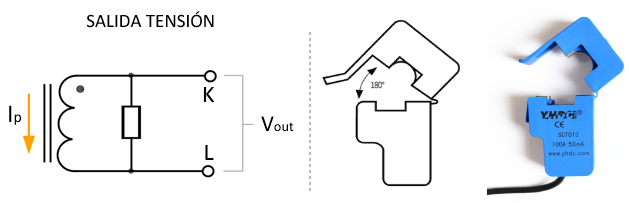
\includegraphics[width=0.9\textwidth]{./Figures/consumo1.png}
\caption{Circuito y pinza del sensor de corriente. }
\label{fig:consumo1}
\end{figure}

La precisión del sensor puede ser del 1\% a 2\%, pero para ello es muy importante que el núcleo ferromagnético se cierre adecuadamente. Hasta un pequeño hueco de aire puede introducir desviaciones del 10\%. Como desventaja, al ser una carga inductiva, el SCT-013 introduce una variación del ángulo de fase cuyo valor es función de la carga que lo atraviesa, pudiendo llegar a ser de hasta 3º \citep{WEBSITE:9}.

Los sensores SCT-013 son pequeños transformadores de corriente o CT (\emph{Current transformartor}) instrumentos ampliamente empleados como elementos de medición. Un transformador de corriente es similar a un transformador de tensión y está basado en los mismos principios de funcionamiento. Sin embargo, persiguen objetivos diferentes \citep{WEBSITE:9}.

Los sensores de la serie SCT-013 son sensores que trabajan como transformadores, la corriente que circula por el cable que se desea medir actúa como el devanado primario (1 espira) e internamente tiene un devanado secundario que dependiendo del modelo puede tener hasta más de 2000 espiras. La cantidad de espiras representa la relación entre corriente que circula por el cable y la que el sensor nos entrega, esta relación o proporción es lo que marca la diferencia entre los diferentes modelos SCT-013, adicionalmente pueden tener una resistencia de carga en la salida y de esta forma en lugar de corriente se trabaja con una salida de tensión \citep{WEBSITE:21}. La figura \ref{fig:espiras} ilustra los devanados mencionados.


\begin{figure}[htpb]
\centering 
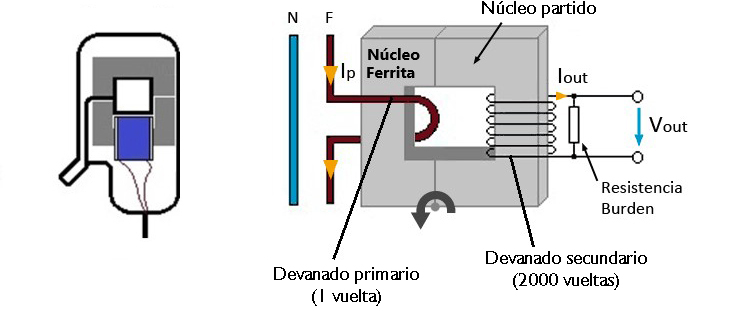
\includegraphics[width=1.0\textwidth]{./Figures/espiras.jpg}
\caption{Partes del núcleo ferromagnético del sensor de corriente.}
\label{fig:espiras}
\end{figure}

La relación de transformación de intensidad se expresa entre el número de espiras, como se muestra en ecuación \ref{eq:proporcionform}.

\begin{equation}
	\label{eq:proporcionform}
	\left( \frac{Is}{Ip} \right)=\left( \frac{Vp}{Vs} \right)=\left( \frac{Np}{Ns} \right)
\end{equation}

A esto se le llama relación de transformación. Relaciona el número de espiras del devanado primario (Np), del devanado secundario (Ns), las intensidades del primario (Ip), del secundario (Is), el tensión del primario (Vp) y del secundario (Vs). 


Para utilizar el sensor SCT-013 no es necesario interrumpir (cortar o desempalmar) el cable que vamos a medir, porque al igual que una pinza amperimétrica tiene el núcleo partido. Si pasamos por ejemplo los dos cables de una conexión monofásica, nuestra lectura será 0, puesto que los cables tienen corrientes opuestas \citep{WEBSITE:21}. La figura \ref{fig:conectacorrecto} ilustra la forma correcta de uso del sensor.
\vspace{0.5cm}
\begin{figure}[htpb]
\centering 
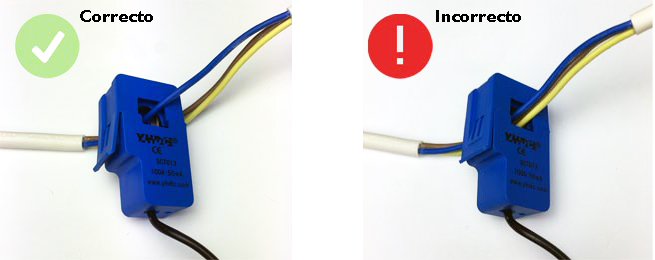
\includegraphics[width=0.8\textwidth]{./Figures/correcto.jpg}
\caption{Forma de uso del sensor de corriente \protect\footnotemark.}
\label{fig:conectacorrecto}
\end{figure}

\footnotetext{Imagen de \url{https://programarfacil.com/blog/arduino-blog/sct-013-consumo-electrico-arduino/}}


A diferencia de los transformadores de tensión, en un transformador de intensidad el circuito secundario nunca debería estar abierto, porque las corrientes inducidas podrían llegar a dañar el componente. Por ese motivo, los sensores de SCT-013 disponen de protecciones (resistencia de Burden en los sensores de salida por tensión, o diodos de protección en los sensores de salida por corriente)\citep{WEBSITE:9}.

El proceso de ensamblado se ilustra en las fotografías de la figura \ref{fig:armadoactuador}.

\begin{figure}[htpb]
\centering 
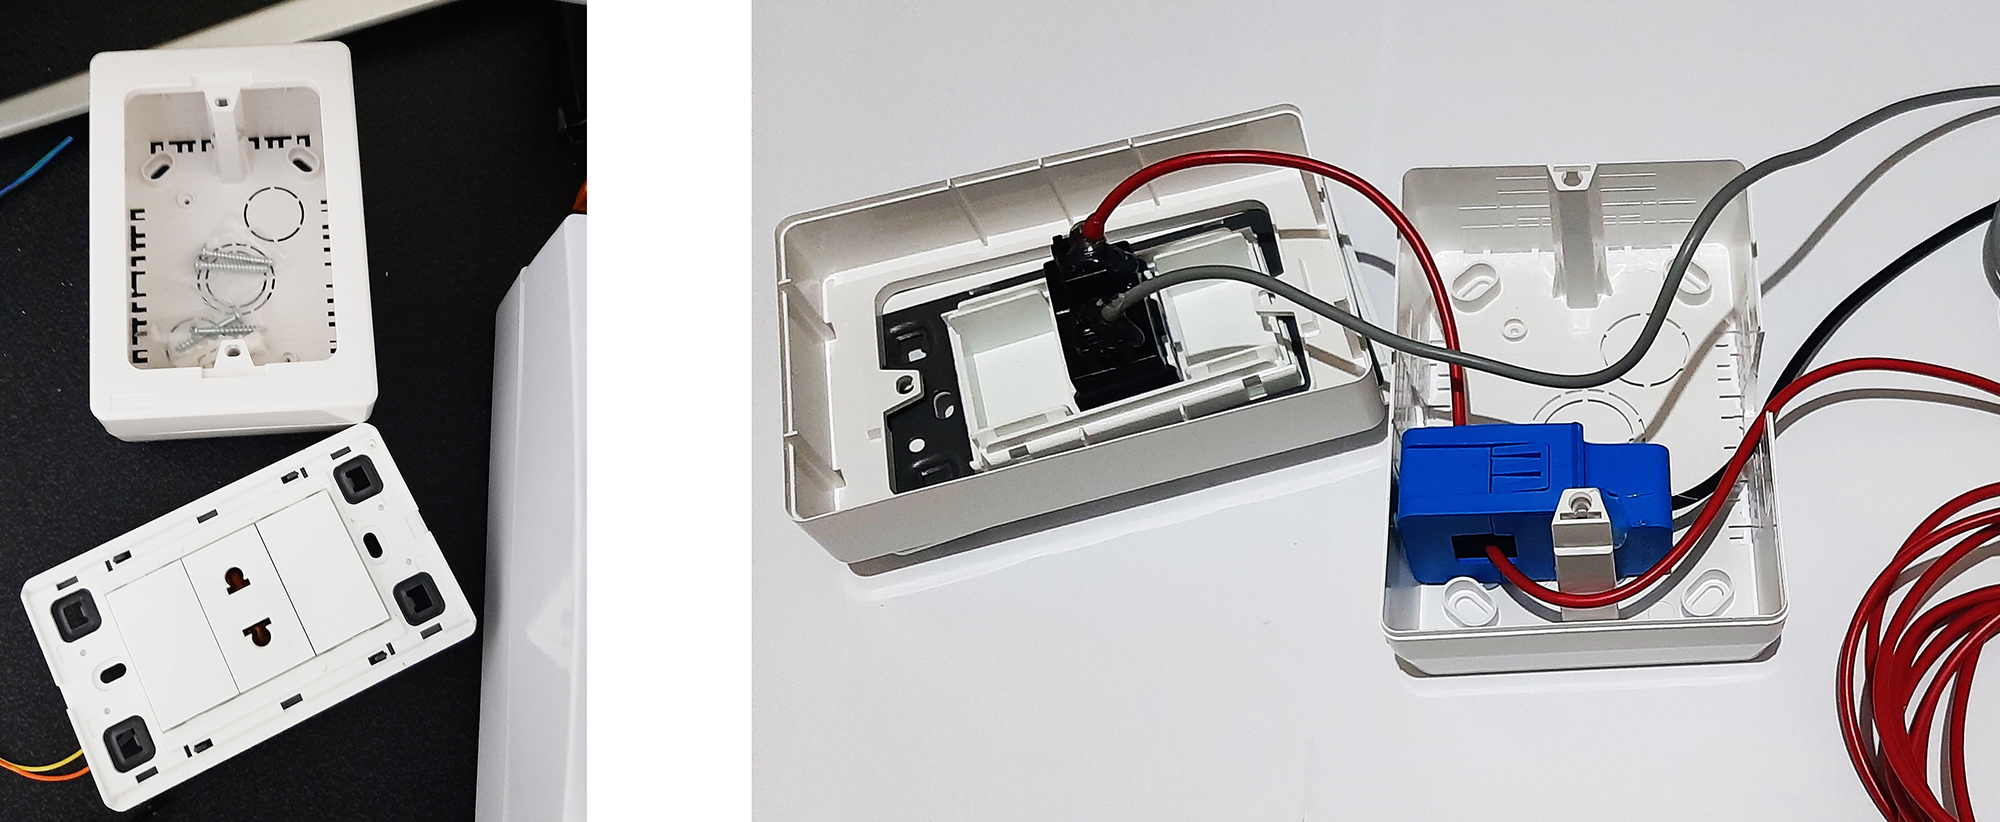
\includegraphics[width=0.85\textwidth]{./Figures/armadoactuador.jpg}
\caption{Ensamblado del módulo actuador. }
\label{fig:armadoactuador}
\end{figure}

\item  \keyword{Aplicación del sensor de tensión eléctrica AC - ZMPT101B}

El sensor transformador de tensión alterno ZMPT101B permite medir tensión alterna como la que se dispone en nuestros hogares (en Perú: 220 VAC - 60 Hz), esta tensión AC no puede ser medida directamente por el ADC de nuestro circuito o placa pues escapa al rango de entrada (0 V a 5 V). El módulo ZMPT101B soluciona el problema reduciendo la tensión AC de entrada a una tensión menor que pueda ser leído por el Arduino, NodeMCU o cualquier otro microcontrolador. La figura \ref{fig:sensortension} ilustra la forma de conexión del módulo sensor a la línea eléctrica doméstica.

El sensor está integrado por un transformador que cumple la función de aislador galvánico para mayor seguridad en el uso. El lado primario del transformador se conecta a la tensión alterna que se desea medir, por ejemplo: la red eléctrica de un hogar de 220 VAC. En el lado secundario del transformador se encuentra un divisor de tensión y un circuito con amplificador operacional (OPAMP LM358) para adicionar un desplazamiento (\emph{offset}) a la salida análoga \citep{WEBSITE:22}. 

\begin{figure}[htpb]
\centering 
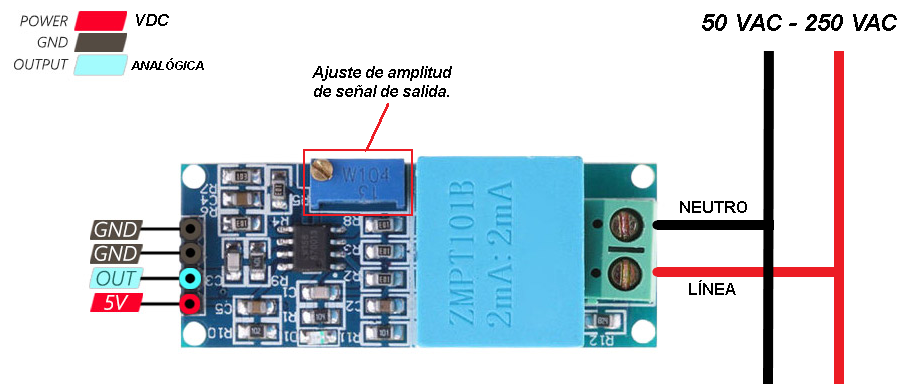
\includegraphics[width=0.85\textwidth]{./Figures/sensortension.png}
\caption{Conexión y partes del sensor de tension.}
\label{fig:sensortension}
\end{figure}


Este sensor soporta una tensión de entrada de hasta 250 VAC y entrega una onda senoidal de amplitud regulable por un potenciómetro en placa. La onda senoidal de salida está desplazada positivamente para que la onda no tenga tensiones negativas y así poder leer la onda completamente con el ADC. El desplazamiento depende de la tensión con la que alimentemos el módulo sensor: si la tensión de alimentación es de 5 V el desplazamiento será de 2.5 V y si se alimenta el módulo con 3.3 V el desplazamiento será de 1.65 V \citep{WEBSITE:23}. Su circuito de acondicionamiento de señal interno permite que la tensión de salida del módulo sensor pueda ser leído por cualquier microcontrolador con entrada analógica (ADC), de esta forma es posible leer la tensión instantánea y realizar cálculos de energía, como: tensión pico a pico (Vpp) y tensión eficaz (Vrms). 

Debido a la naturaleza de los transformadores solo puede medir tensión AC \citep{WEBSITE:22} \citep{ARTICLE:1}. Para su uso con la tarjeta NodeMCU ESP8266, los extremos son 0 y 3.3 V con una compensación de 1.65 V. La figura \ref{fig:ondas} muestra el desplazamiento de onda senoidal.


\begin{figure}[htpb]
\centering 
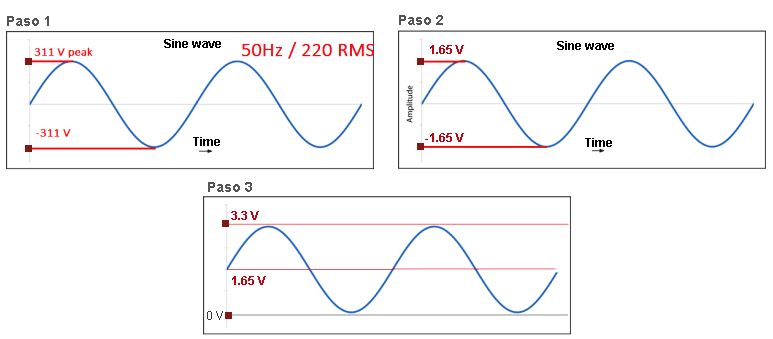
\includegraphics[width=1.02\textwidth]{./Figures/ondas.png}
\caption{Señal del ZMPT101B con el NodeMCU ESP8266 \protect\footnotemark.}
\label{fig:ondas}
\end{figure}

\footnotetext{Imagen tomada de \url{https://surtrtech.com/2020/04/08/}}
\vspace{1.0cm}
\item \keyword{Medición del consumo eléctrico}

Para determinar la potencia eléctrica consumida, el sistema recolecta mediciones del sensor de consumo y realiza la operación matemática de la formula \ref{eq:potenciaform} y los resultados los almacena de forma periódica en la base de datos local y remota. Los datos son agrupados según la hora de lectura junto a su respectiva fecha. La tabla \ref{tab:tablaconsumos} muestra la lógica de registros.

\begin{table}[h]
	\centering
	\caption[Registros de consumos]{Registros de consumos}
	\begin{tabular}{l c c c}    
		\toprule
		\textbf{Potencia electrodoméstico} 	 & \textbf{formato}  & \textbf{respaldo} &\textbf{fecha} \\
		\midrule
		P. consumo ventilador (pcv) & agrupacion (a1) & 10:00 am & 01/02/2022\\		
		P. consumo ventilador (pcv)& agrupacion (a2) & 11:00 am &01/02/2022 \\
		P. consumo ventilador (pcv)& agrupacion (a3) & 2:00 pm & 01/02/2022\\		
		P. consumo ventilador (pcv)& agrupacion (a4) & 3:00 pm & 01/02/2022\\		
		
		\bottomrule
		\hline
	\end{tabular}
	\label{tab:tablaconsumos}
\end{table}

Considerando como ejemplo los datos de la tabla \ref{tab:tablaconsumos}, el consumo del ventilador en el día 01/02/2022 será la sumatoria de las agrupaciones. La formula \ref{eq:potenciaformejemplo} muestra la operación.
\begin{equation}
	\label{eq:potenciaformejemplo}
	Consumo Total = \left( pcv(a1) + pcv(a2)+ pcv(a3)+ pcv(a4) \right)
\end{equation}
La formula \ref{eq:potenciaformejemplo} es equivalente a la formula \ref{eq:potenciaformejemplo2} para las horas de uso, según el ejemplo citado.
\begin{equation}
	\label{eq:potenciaformejemplo2}
	Consumo Total = \left(Potencia Consumida Ventilador X 4 Horas Uso \right)
\end{equation}

Los valores del consumo total serán usados para generar la facturación mensual por consumo eléctrico. La figura \ref{fig:modconsumo} muestra la construcción del módulo de consumo.


\end{enumerate}
\subsection{Módulo réplica}
Este módulo contiene una copia del software de monitoreo y control pero con la diferencia que se ejecuta en la nube usando los servicios de un servidor y un broker remoto.

%%%%%%%%%%%%%%%%%%%%%%%%%%%%%%%%%%%%%%%%%%%%%%%%%%%%%%%%%%%%%%%%%%%%%%%%%%%%%
\begin{landscape} % esto es para rotar la pagina e imagen
\begin{figure}[htpb]
\centering 
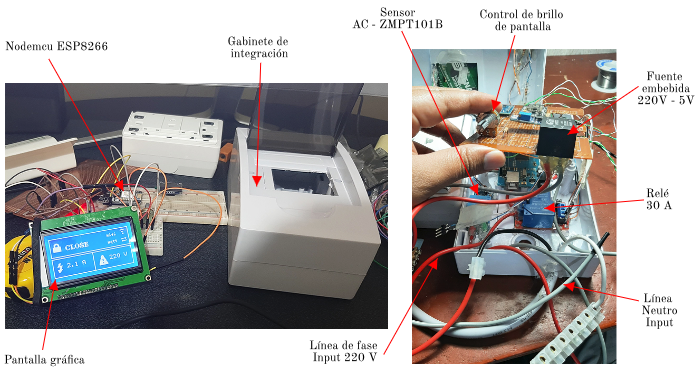
\includegraphics[width=1.5\textwidth]{./Figures/moduloconsumo.png}
\caption{Construcción del módulo de consumo.}
\label{fig:modconsumo}
\end{figure}
\end{landscape} % 
%%%%%%%%%%%%%%%%%%%%%%%%%%%%%%%%%%%%%%%%%%%%%%%%%%%%%%%%%%%%%%%%%%%%%%%%%%%%%%

\section{Configuración de la red WLAN}

El diseño y la configuración de la red WLAN tiene un rol fundamental dentro del desempeño del sistema porque permite garantizar un canal de comunicación más seguro si interferir la red doméstica.

\subsection{Diseño de la red física local}

Para esta tarea se agregó un Router inalámbrico como punto de acceso adicional a la red local, sirviendo como medio de comunicación exclusivo de los sensores y actuadores del sistema dentro de la red interna del hogar o edificio. La figura \ref{fig:diagramared} ilustra el diseño física de la red utilizada.


\subsection{Configuración del Router inalámbrico}
Los principales criterios de configuración a considerar del router inalámbrico son la seguridad de la señal y la elección del canal para la comunicación Wi-Fi. Para el presente trabajo usamos un \emph{Router/Access Point} de alta ganancia 300 MBPS SATRA, porque ofrece tasas de transferencia de datos de 300Mbps y garantiza una cobertura inalámbrica sin cortes tanto en la red del hogar como de la oficina y es compatible con el estándar de encriptación WPA2 (\emph{Wi-Fi Protected Access 2}), diseñado para proteger a la red de ataques externos en un nivel mas alto \citep{WEBSITE:25}. La figura \ref{fig:router} muestra el modelo del router SATRA.

\begin{figure}[htpb]
\centering 
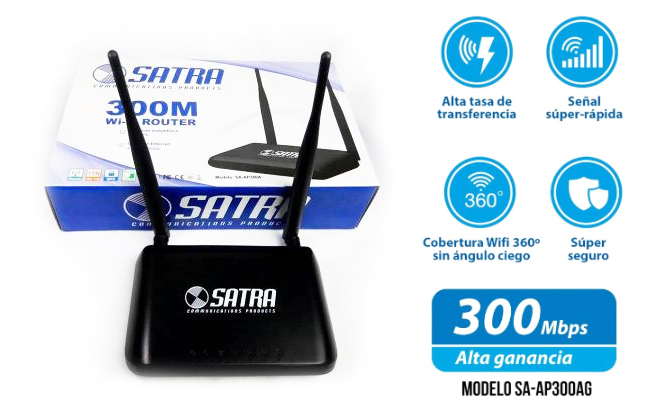
\includegraphics[width=0.7\textwidth]{./Figures/router.jpg}
\caption{Modelo del router utilizado para el diseño de red.}
\label{fig:router}
\end{figure}

Este router tiene tres formas de funcionamiento: access point, router y repetidor. Para nuestro trabajo se seleccionó la configuración Access Point (AP) o punto de acceso. La figura \ref{fig:funcionamientorouter} muestra la configuración del modo de funcionamiento.

Al crear y configurar una red inalámbrica WLAN, nos encontramos con uno de los problemas más comunes con las redes WiFi, el solapamiento de canales, debido a la gran cantidad de equipos que funcionan en la banda de frecuencia de 2,4 GHz. La mala configuración de red puede ser un motivo para problemas de comunicación Wi-Fi. La conexión a Internet lenta y las desconexiones pueden ocurrir si la red inalámbrica no está configurada correctamente o si hay demasiados dispositivos que están compitiendo por el espacio aéreo inalámbrico de la red. Cada equipo WiFi que cumple con el estándar 802.11 b/g utiliza uno de los 13 canales establecidos de 14 en total y si 2 o más equipos cercanos utilizan el mismo canal, se produce el solapamiento. 

%%%%%%%%%%%%%%%%%%%%%%%%%%%%%%%%%%%%%%%%%%%%%%%%%%%%%%%%%%%%%%%%%%%%%%%%%%%%%
\begin{landscape} % esto es para rotar la pagina e imagen
\begin{figure}[htpb]
\centering 
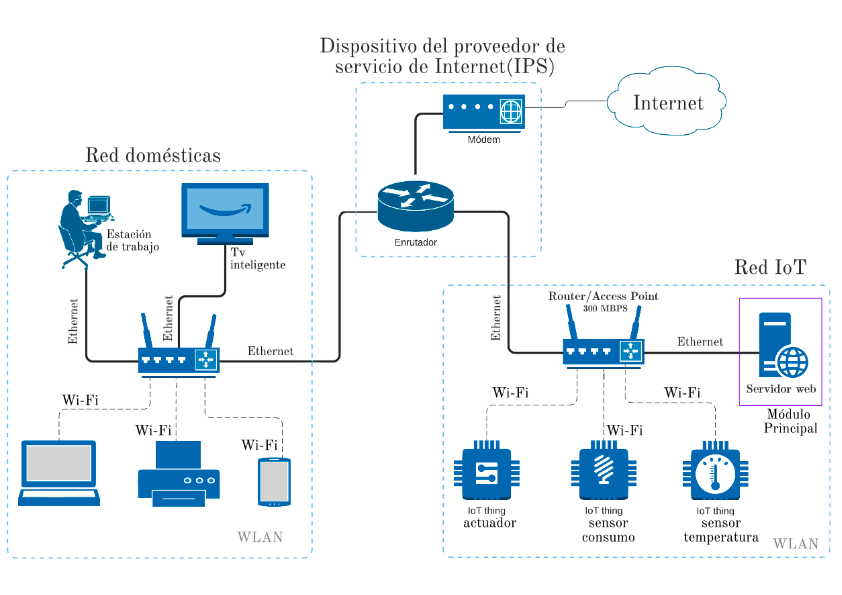
\includegraphics[width=1.3\textwidth]{./Figures/rediot.png}
\caption{Diseño físico de la red WLAN para el sistema IoT.}
\label{fig:diagramared}
\end{figure}
\end{landscape} % 
%%%%%%%%%%%%%%%%%%%%%%%%%%%%%%%%%%%%%%%%%%%%%%%%%%%%%%%%%%%%%%%%%%%%%%%%%%%%%%

Cada canal ocupa un ancho de banda de 22 MHz. El efecto del solapamiento es la bajada en el rendimiento (velocidad) de las redes afectadas \citep{WEBSITE:26}.

\begin{figure}[htpb]
\centering 
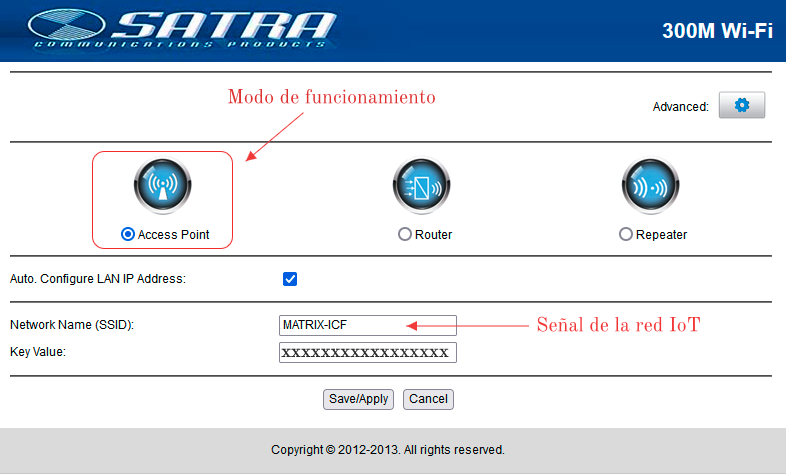
\includegraphics[width=0.7\textwidth]{./Figures/funcionamientorouter.png}
\caption{Elección del modo de funcionamiento del router.}
\label{fig:funcionamientorouter}
\end{figure}

El figura \ref{fig:canales} muestra el ancho de banda utilizado por cada canal y el solapamiento que se produce entre ellos \citep{WEBSITE:27}.

\begin{figure}[htpb]
\centering 
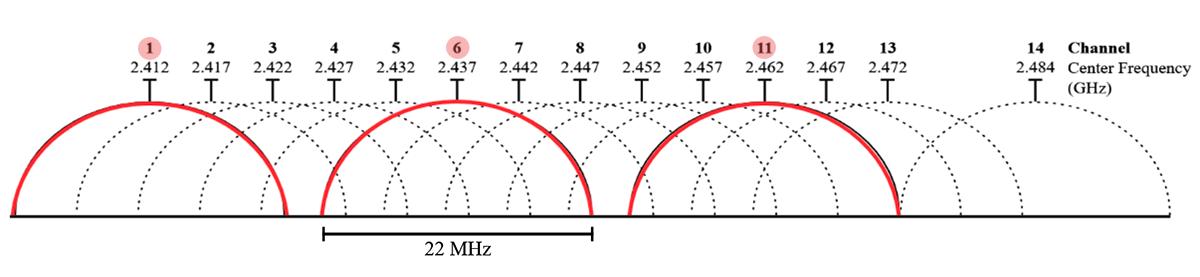
\includegraphics[width=1.0\textwidth]{./Figures/canales.png}
\caption{Diagrama de los canales de 2.4 GHz.}
\label{fig:canales}
\end{figure}

\subsubsection{Elección del canal de comunicación}
En la banda de 2,4 GHz, que por lo general es \emph{Wireless-N}, siempre se elije el canal 1, 11 o 6. Los canales distintos de 1, 11 o 6 recibirán más interferencias. 

Para la elección del canal se tomo en cuenta la figura  \ref{fig:canales} y las siguientes consideraciones \citep{WEBSITE:28}:

\begin{itemize}
\item El canal 1 interferirá y recibirá interferencias de los canales 1-5 de  2,4 GHz.
\item El canal 6 interferirá y recibirá interferencias de los canales 2-10 de  2,4 GHz.
\item El canal 11 interferirá y recibirá interferencias de los canales 7-13 de 2,4 GHz.
\end{itemize}

Utilizando la información anterior, se puede observar que siempre se debe elegir los canales 1, 11 o 6. Si se hace lo contrario, se tendrá la interferencia de más de un canal inalámbrico principal de 2,4 GHz \citep{WEBSITE:28}, ocasionando solapamiento o interferencia en el canal de comunicación de la red IoT a utilizar. Sin embargo, es posible que no se pueda acceder a un canal no interferible, porque pueden existir redes Wi-Fi que estén ocupando los canales 1, 6 y 11. Incluso, pueden existir otras redes vecinas que utilicen canales que se solapen parcialmente y para estos casos, se debe buscar un canal donde el impacto de ese solapamiento sea mínimo \citep{WEBSITE:27}.

Pare este trabajo la elección del número de canal se fundamentó en la investigación antes mencionada y en la exploración de las redes Wi-Fi vecinas existentes en el entorno donde se implantó el sistema IoT.

\subsubsection{Elección del ancho de banda del canal}

Para la elección de la anchura del canal se establece en 20 MHz para la banda de 2,4 GHz y en Automático o en todos los anchos (20 MHz, 40 Mhz y 80 MHz) para la banda de 5 GHz \citep{WEBSITE:29}. La anchura del canal especifica el tamaño del ``cauce'' disponible para transferir datos. Los canales más anchos son más rápidos, pero más propensos a sufrir interferencias y a interferir con otros dispositivos. Los 20 MHz para la banda de 2,4 GHz ayudan a evitar problemas de rendimiento y fiabilidad, especialmente cerca de otras redes Wi-Fi y dispositivos de 2,4 GHz, incluidos los dispositivos Bluetooth \citep{WEBSITE:29}. La figura \ref{fig:configuracioncanal} muestra los valores por defecto que tiene el router utilizado y la figura \ref{fig:solapamiento} muestra el solapamiento de las redes inalámbricas locales y vecinas donde se probó el sistema IoT.

\begin{figure}[htpb]
\centering 
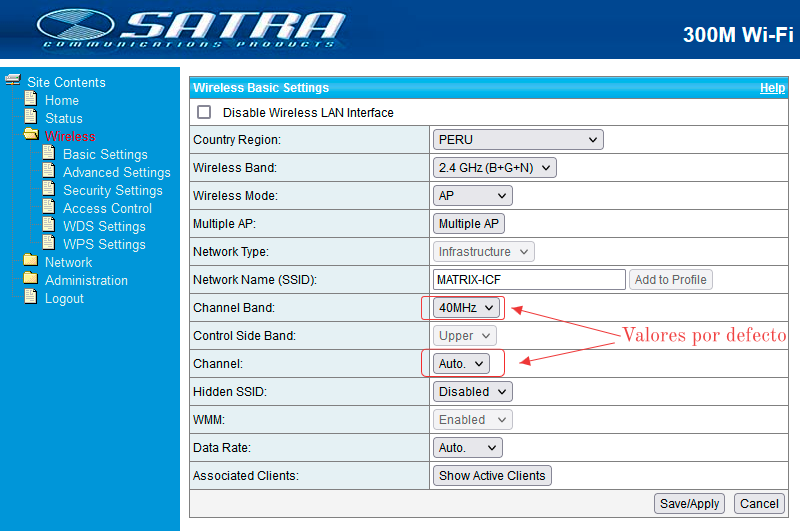
\includegraphics[width=0.9\textwidth]{./Figures/configuracioncanal.png}
\caption{Configuración por defecto del router SATRA.}
\label{fig:configuracioncanal}
\end{figure}

Para los casos donde se amplía el canal (40 MHz), eso significa duplicar las interferencias con las redes vecinas. Para remediarlo, la IEEE introdujo un mecanismo de coexistencia en 2,4 GHz para evitar las molestias a las redes vecinas, muchos fabricantes de routers se han adaptado a la norma, por lo que no permiten que los usuarios seleccionen arbitrariamente los 40 MHz, sino que se limitan a un ``auto 20/40''. Por lo tanto el router sólo utilizará 40 MHz si los canales vecinos están libres de lo contrario, utilizará 20 MHz para no solapar las redes vecinas \citep{WEBSITE:30}.

La figura \ref{fig:configuracionancho} muestra la configuración final elegida para este trabajo. Las pruebas y análisis de canales así como la justificación para su elección se describen en el capitulo 4 de este documento.

%%%%%%%%%%%%%%%%%%%%%%%%%%%%%%%%%%%%%%%%%%%%%%%%%%%%%%%%%%%%%%%%%%%%%%%%%
\begin{landscape} % esto es para rotar la pagina e imagen
\begin{figure}[htpb]
\centering 
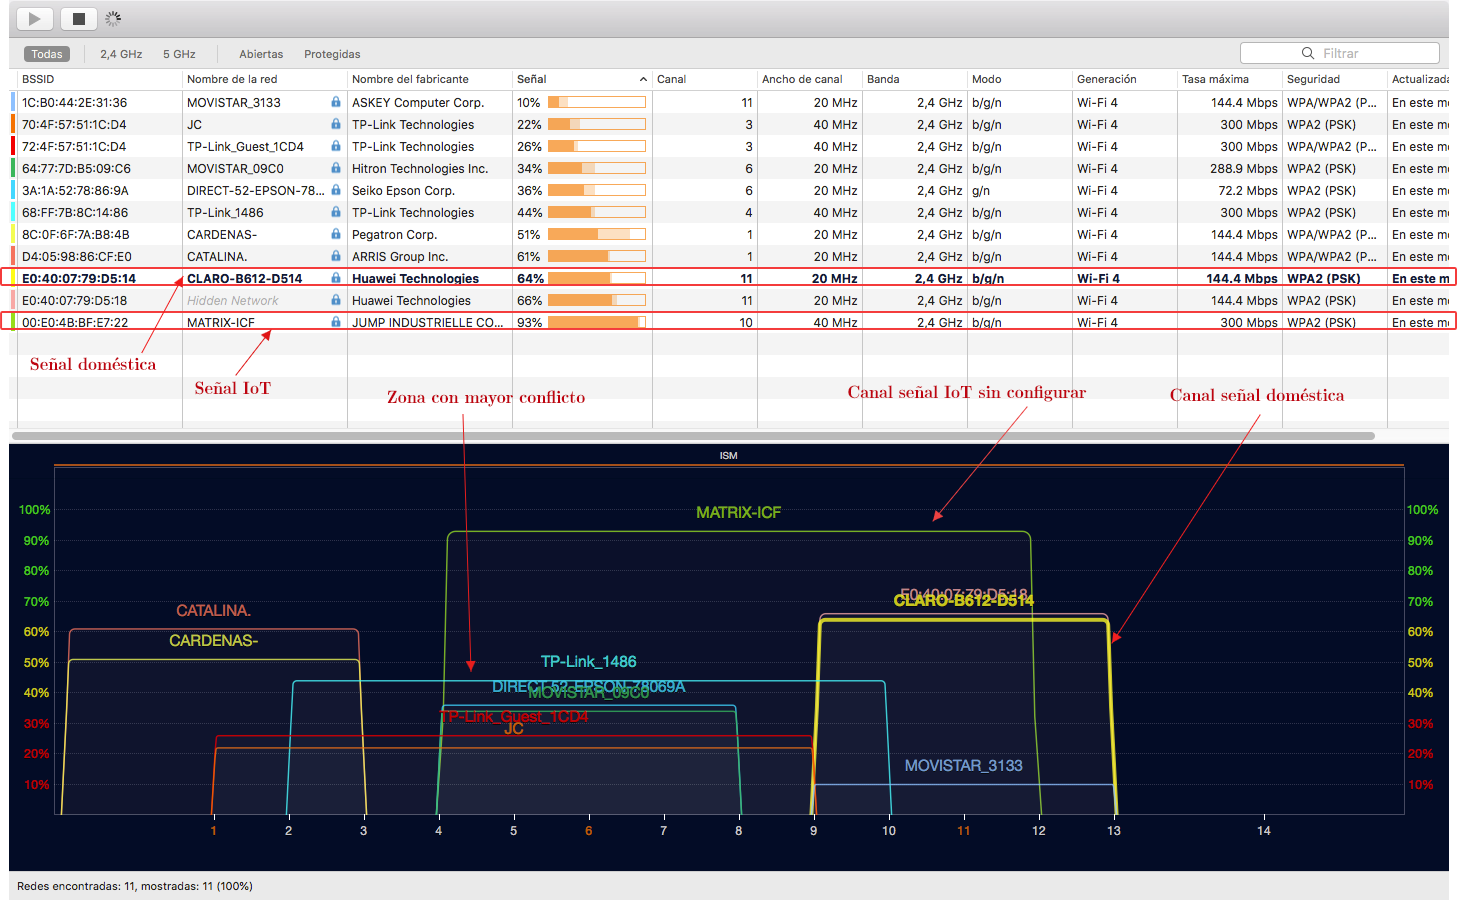
\includegraphics[width=1.5\textwidth]{./Figures/wifi/01-doc.png}
\caption{Solapamiento de canales de las redes inalámbricas locales y vecinas.}
\label{fig:solapamiento}
\end{figure}
\end{landscape} % 
%%%%%%%%%%%%%%%%%%%%%%%%%%%%%%%%%%%%%%%%%%%%%%%%%%%%%%%%%%%%%%%%%%%%%%%%%%%%

\begin{figure}[htpb]
\centering 
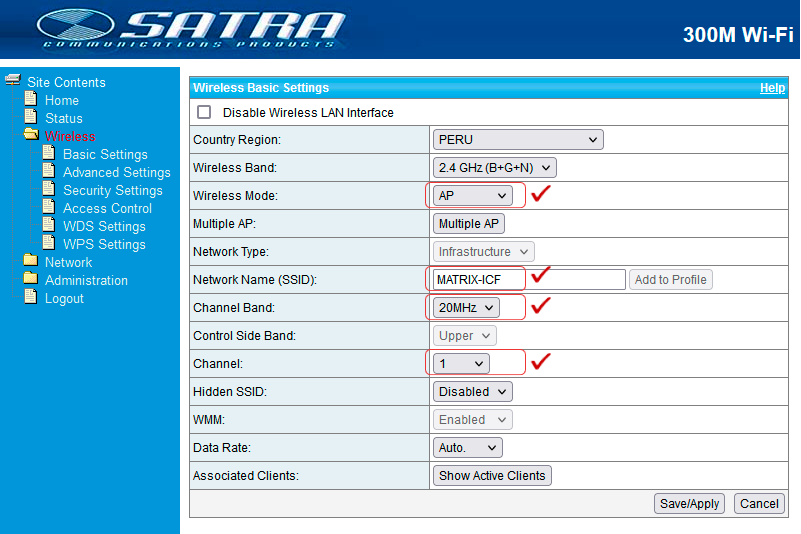
\includegraphics[width=0.9\textwidth]{./Figures/configuracionancho.png}
\caption{Configuración para la red WLAN del sistema IoT.}
\label{fig:configuracionancho}
\end{figure}
%------------------------------------------------

\subsubsection{Configuración de seguridad inalámbrica}
Dentro de los parámetros de seguridad se configuró la opción de autenticación (\emph{auth. and encryption}). La figura \ref{fig:encriptacion} ilustra la elección de encriptación y autenticación para el acceso a la señal del access point y en la figura \ref{fig:configuracionfinal} Ilustra los resultados finales de la configuración del access point.

%\vspace{0.1cm}
\begin{figure}[htpb]
\centering 
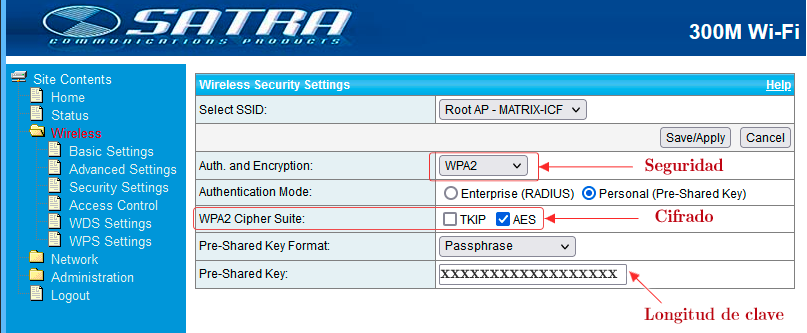
\includegraphics[width=1.0\textwidth]{./Figures/encriptacion.png}
\caption{Configuración de autenticación para la señal Wi-Fi.}
\label{fig:encriptacion}
\end{figure}
%------------------------------------------------------
%\vspace{0.1cm}
\begin{figure}[htpb]
\centering 
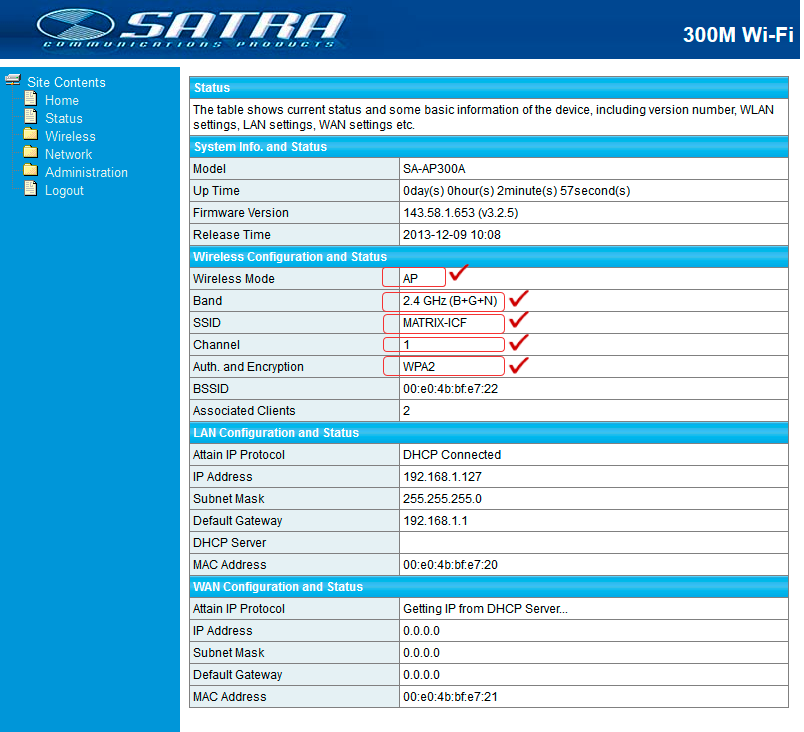
\includegraphics[width=1.0\textwidth]{./Figures/configuracionfinal.png}
\caption{Resumen de la configuración resultante del router.}
\label{fig:configuracionfinal}
\end{figure}

\section{Software a medida para monitoreo y control}

El software desarrollado para este trabajo fue hecho a medida por ser parte fundamental dentro de los objetivos planteados al inicio, como emprendimiento personal. 

El software es de tipo web y cumple con la característica de ser responsivo para garantizar la adaptación visual a distintos dispositivos del mercado actual. La figura \ref{fig:software1} y \ref{fig:software2} muestran los resultados responsivos para cada tipo de dispositivo considerado en el desarrollo.

\begin{figure}[htpb]
\centering 
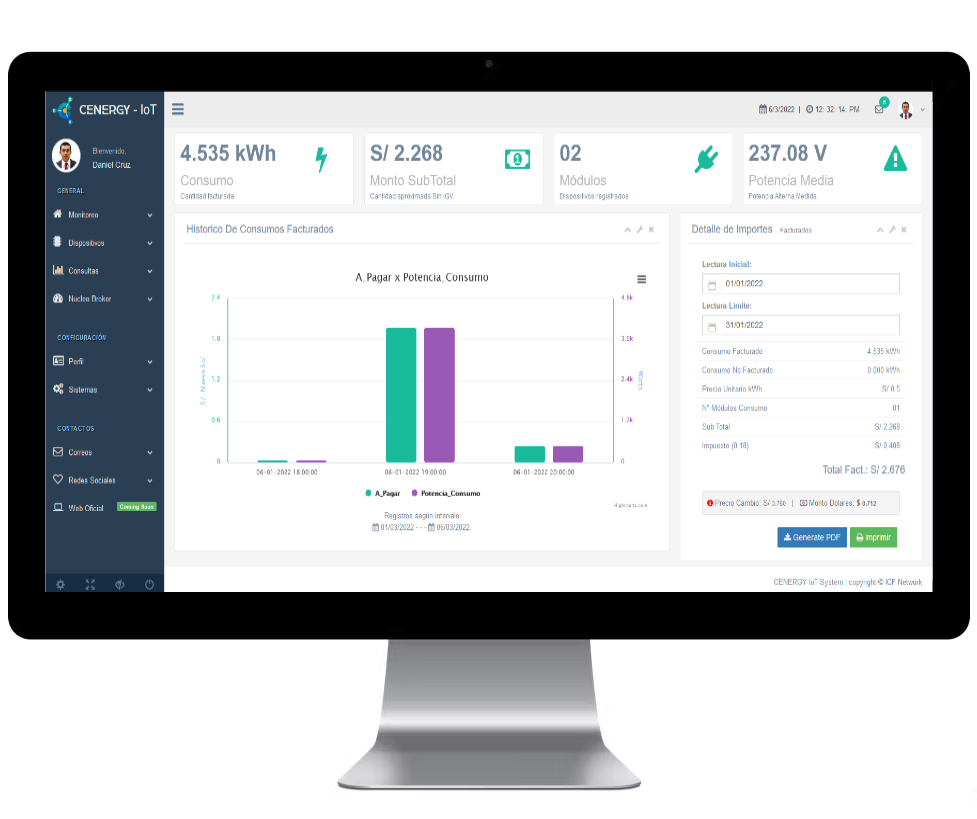
\includegraphics[width=0.65 \textwidth]{./Figures/responsive1.png}
\caption{Vista del software en equipos desktop y laptop.}
\label{fig:software1}
\end{figure}

\vspace{1.0cm}
\begin{figure}[htpb]
\centering 
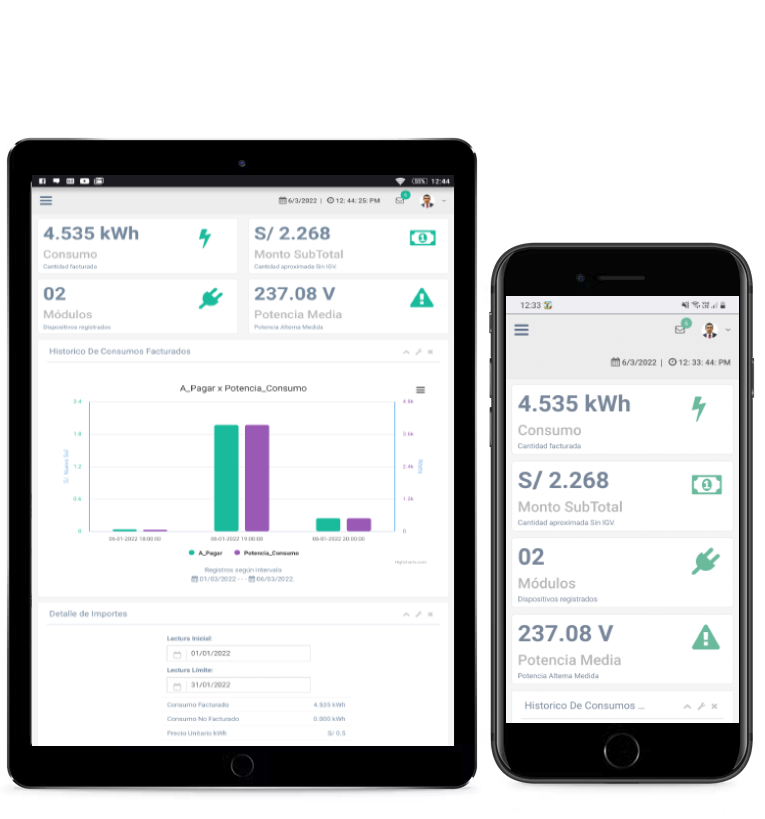
\includegraphics[width=0.6\textwidth]{./Figures/responsive2.png}
\caption{Vista del software en tableta y celular.}
\label{fig:software2}
\end{figure}

\vspace{1.0cm}
\section{Resultados de los módulos del sistema IoT}
En esta sección se muestran las imágenes reales de los resultados obtenidos de la construcción de cada módulo físico. Estos dispositivos fueron utilizados para las pruebas de validación en un ambiente real IoT. Las figuras \ref{fig:modPrincipal}, \ref{fig:modTemp} y \ref{fig:modConsumo2} muestran los módulos.

 
\begin{figure}[htpb]
\centering 
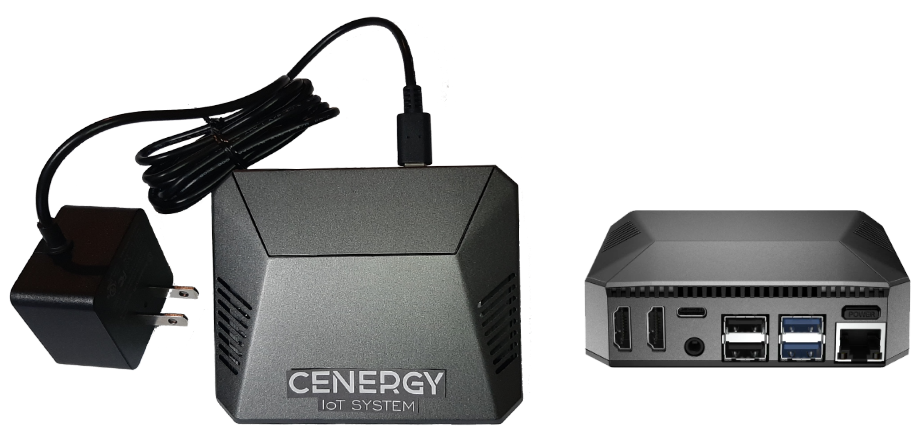
\includegraphics[width=0.9\textwidth]{./Figures/principal2.png}
\caption{Vista superior y posterior del módulo principal.}
\label{fig:modPrincipal}
\end{figure}



\begin{figure}[htpb]
\centering 
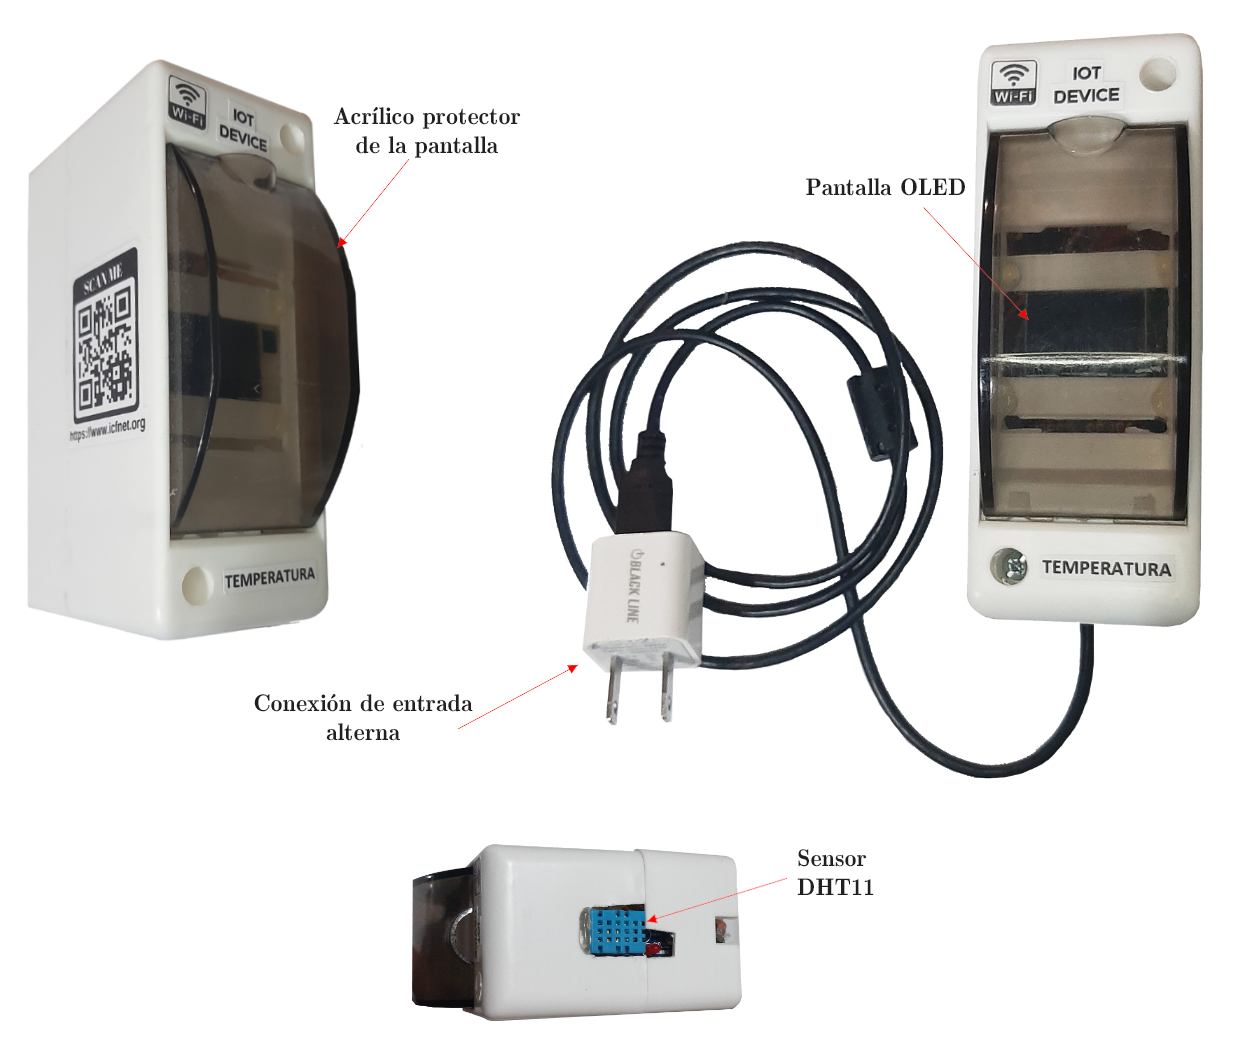
\includegraphics[width=0.85\textwidth]{./Figures/moduloTemp2.png}
\caption{Vista lateral, frente y superior del módulo de temperatura.}
\label{fig:modTemp}
\end{figure}



%%%%%%%%%%%%%%%%%%%%%%%%%%%%%%%%%%%%%%%%%%%%%%%%%%%

\begin{landscape} % esto es para rotar la pagina e imagen
\begin{figure}[htpb]
\centering 
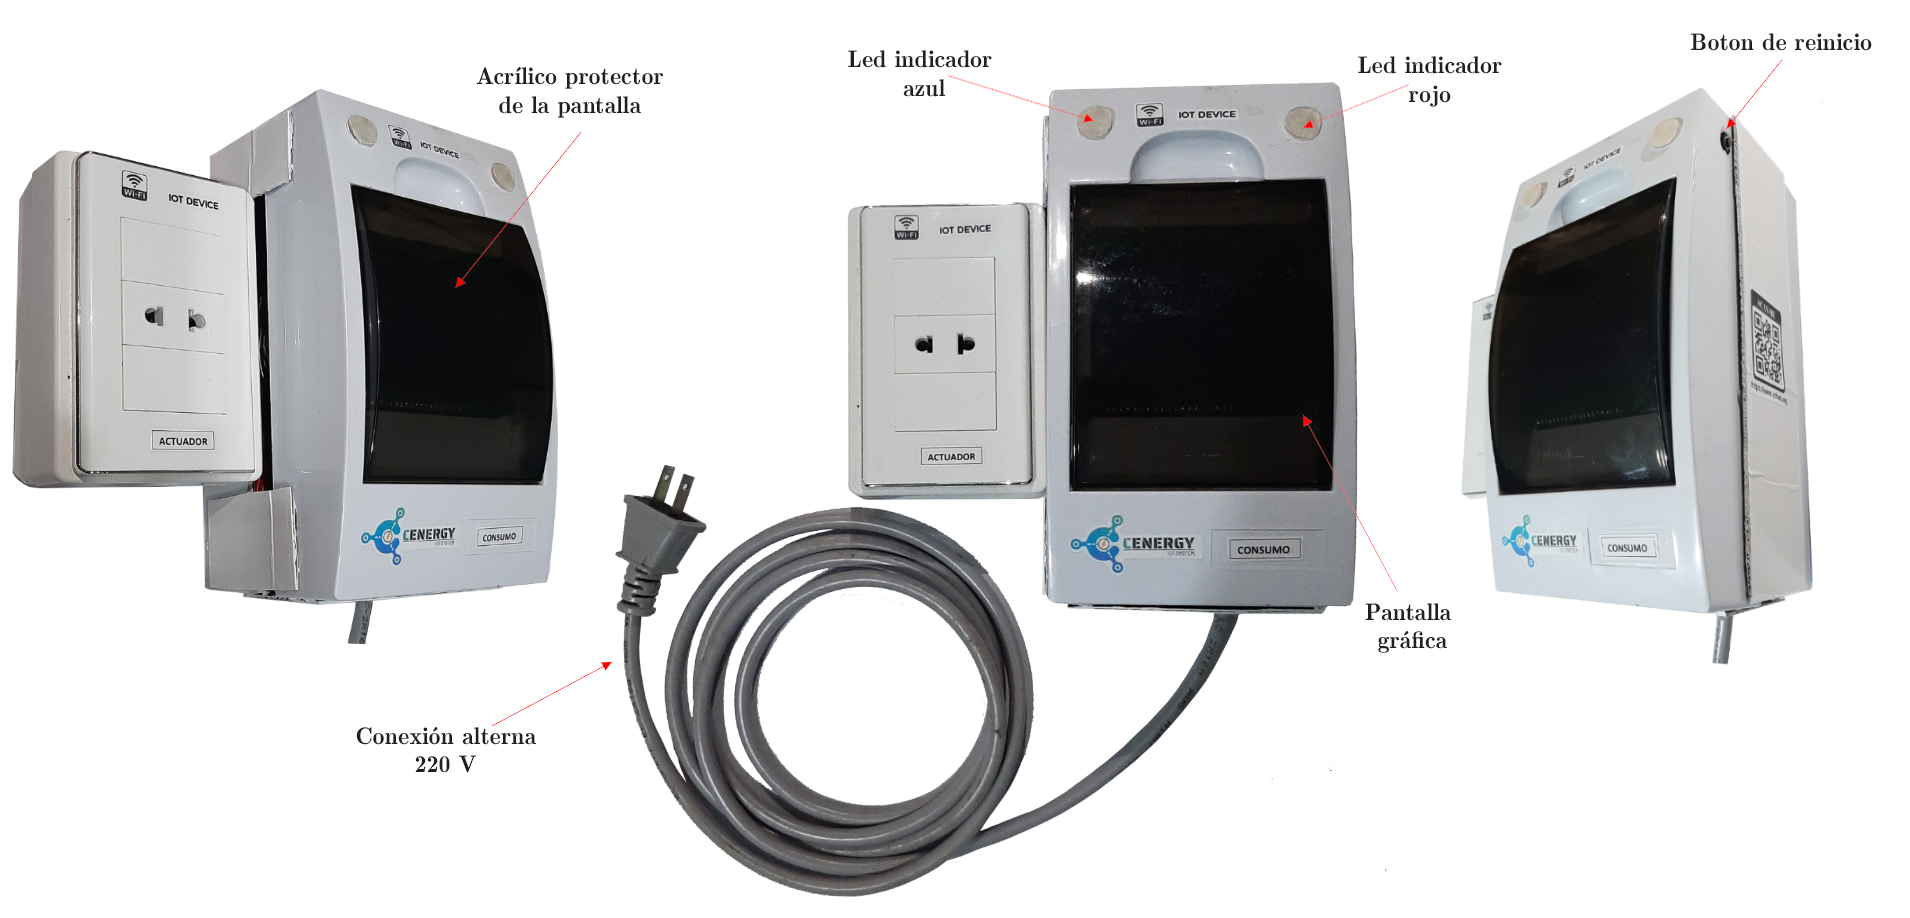
\includegraphics[width=1.8\textwidth]{./Figures/consumo3.png}
\caption{Vista frontal y lateral del módulo actuador y módulo de consumo.}
\label{fig:modConsumo2}
\end{figure}
\end{landscape} %


%%%%%%%%%%%%%%%%%%%%%%%%%%%%%%%%%%%%%%%%%%%%%%%%%%%
\section{Interfaces gráficas del software de monitoreo y control}

El software de monitoreo y control fue diseñado y desarrollado a medida con el objetivo de ser el autor de este trabajo el dueño de los derechos de \emph{Copyright} del mismo, ademas el software por ser de tipo web requiere solo un navegador web y conexión a la red local o a Internet para poder ser utilizado. El software ha sido nombrado como: \emph{Cenergy IoT System} y hace referencia al control de energía eléctrica mediante un sistema IoT. Se espera su evolución y madurez en trabajos futuros. 

%Las principales interfaces gráficas de usuario (GUI) que se muestran a %continuación son el resultado de lo logrado en esta primera versión del %software hasta la fecha de presentación de este trabajo. Las GUIs son:

\begin{itemize}
\item La interfaz de control de acceso al sistema se muestra en la figura \ref{fig:gui0}. Los credenciales utilizados son el numero de su documento nacional de identidad (DNI) y una contraseña de longitud mínima de 8 caracteres.

\item La interfaz de presentación inicial al ingresar al sistema (dashboard) se muestra en la figura \ref{fig:gui1}. Esta interfaz muestra el resumen de lo que actualmente esta almacenado en la base de datos del sistema. Resalta el consumo facturado y el no facturado a la fecha actual de acceso considerando intervalos de un mes.

\item La interfaz de monitoreo para sensores se muestra en la figura \ref{fig:gui2}. Esta interfaz permite mostrar en tiempo real los sensores que tiene el sistema IoT, así como el estado de los mismos. Si un sensor tiene un estado CONECTADO se podrá observar sus detalles desde la opción ``ver detalles'', pudiendo acceder a una vista gráfica más detallada del mismo, tal como se muestra en la figura \ref{fig:gui2-1}.

\item La interfaz de monitoreo y control para sensores de consumo y sus actuadores se muestran el figura \ref{fig:gui3}. Esta interfaz permite visualizar en tiempo real los módulos registrados y conectados al sistema IoT. Cada módulo en estado CONECTADO muestra el dispositivo que esta realizando consumo mediante una onda de señal de energía activa, junto a su interruptor actuador cuya función es el control del paso o limitación de energía eléctrica en el módulo. Si el módulo esta con el estado CONECTADO se podrá observar sus detalles desde la opción ``ver detalles'', pudiendo acceder a una vista gráfica más detallada del mismo, tal como se muestra en la figura \ref{fig:gui3-1}.

\item La interfaz de registro o agregado de módulos al sistema IoT se muestra en la figura \ref{fig:gui4}. Para el registro cada módulo cuenta con un código y numero de módelo, para su identificación dentro del sistema.

\item El software actualmente presenta interfaces para cuatro tipos de consultas, que son: lecturas de temperatura, historial de temperatura, consumo sin facturar y consumo facturado. Cada lectura que se registra en la base de datos se respalda en agrupaciones de intervalos de horas y los registros que aun no completan las horas, podran ser consultados desde las opciones: lectura de temperatura y consumos sin facturar. Los resultados de las consultas podrán ser exportados en formatos excel o pdf y si se desea, ser impresos directamente. La figura \ref{fig:gui5} muestra la interfaz de consultas.

\item El software cuenta con una interfaz que muestra un grafo que permite visualizar en tiempo real la comunicación de los módulos asi como los mensajes entre canales. El grafo se muestra en la figura \ref{fig:grafo}.


\end{itemize}






%%%%%%%%%%%%%%%%%%%%%%%%%%%%%%%%%%%%%%%%%%%%%%%%%%%
\begin{landscape} % esto es para rotar la pagina e imagen
\begin{figure}[htpb]
\centering 
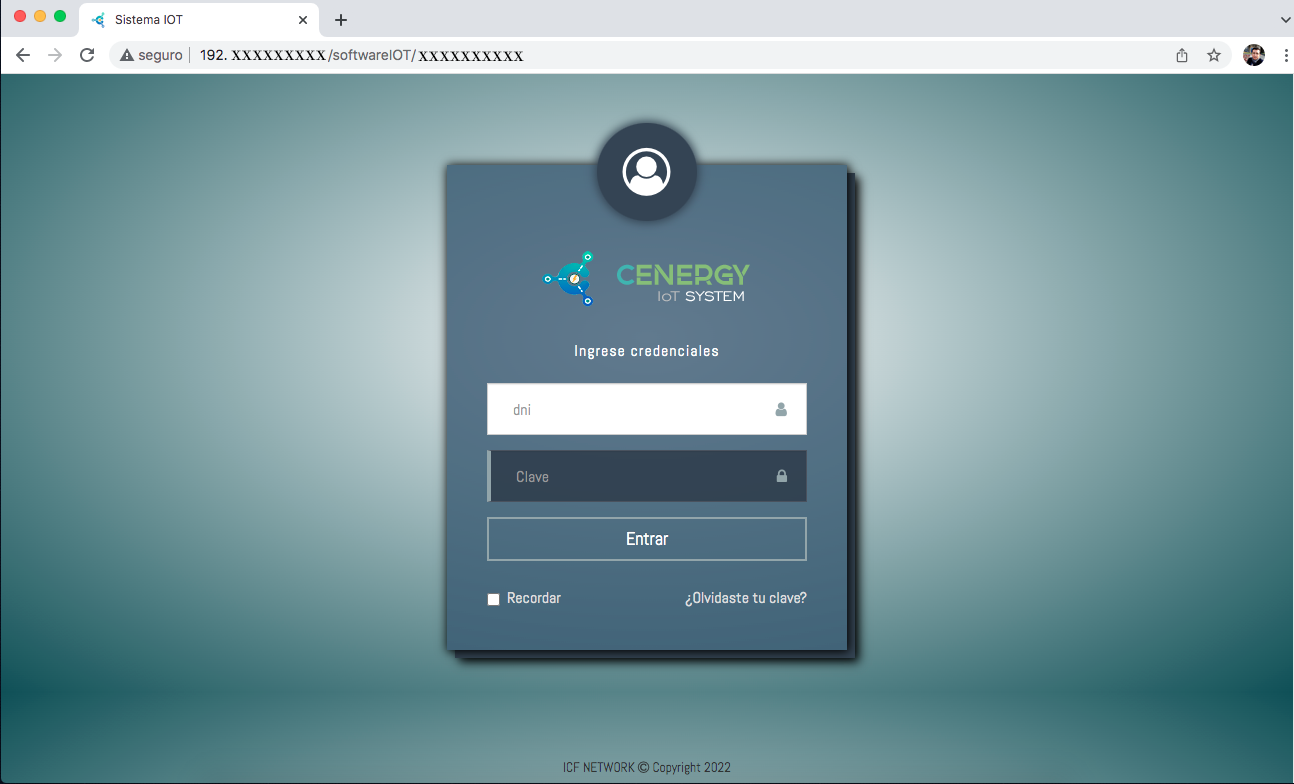
\includegraphics[width=1.55\textwidth]{./Figures/gui/0.png}
\caption{Interfaz gráfica de usuario de acceso al software de monitoreo y control.}
\label{fig:gui0}
\end{figure}
\end{landscape} %

%%%%%%%%%%%%%%%%%%%%%%%%%%%%%%%%%%%%%%%%%%%%%%%%%%%

%%%%%%%%%%%%%%%%%%%%%%%%%%%%%%%%%%%%%%%%%%%%%%%%%%%
\begin{landscape} % esto es para rotar la pagina e imagen
\begin{figure}[htpb]
\centering 
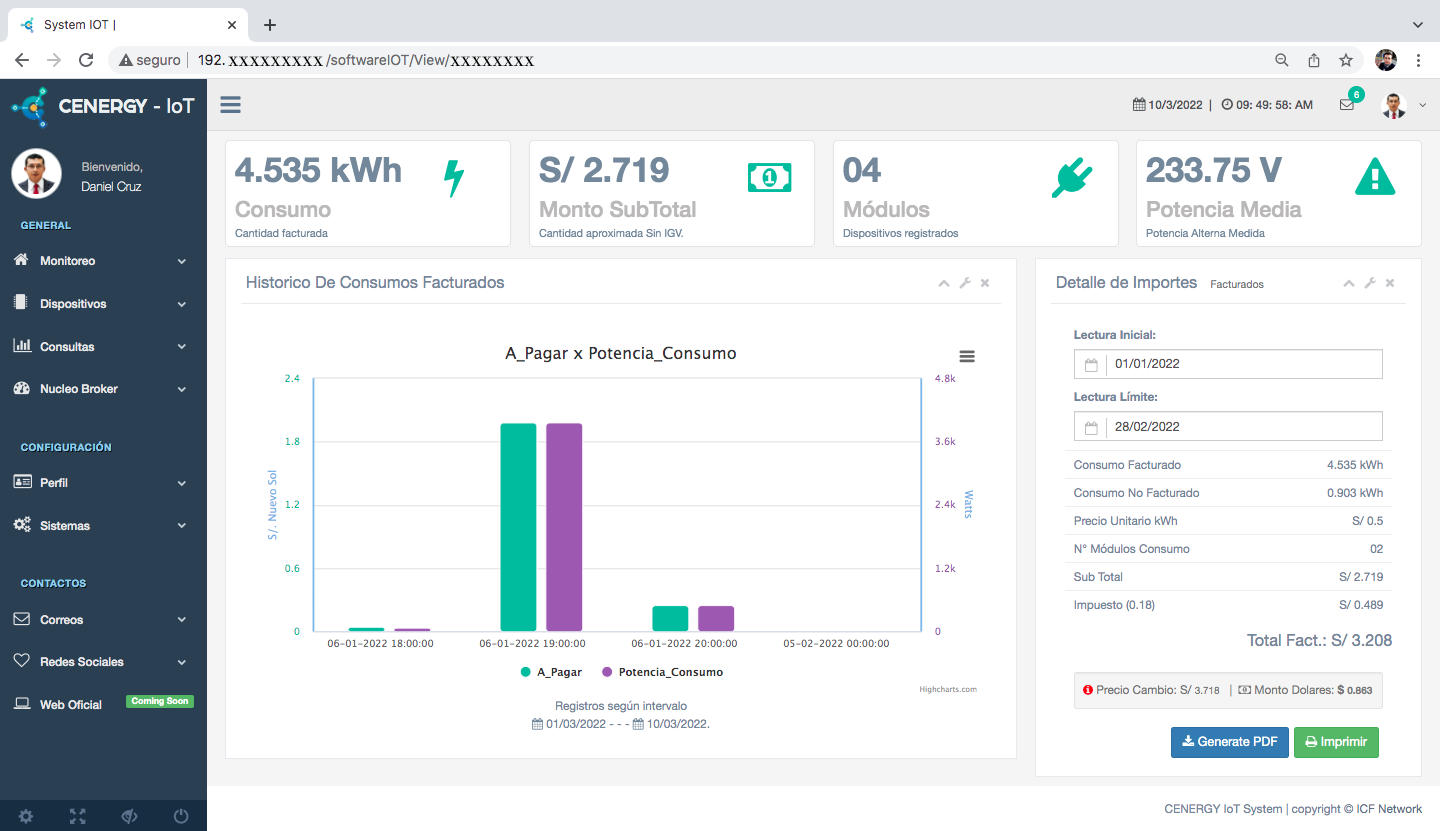
\includegraphics[width=1.55\textwidth]{./Figures/gui/1.png}
\caption{Dashboard inicial del software de monitoreo y control.}
\label{fig:gui1}
\end{figure}
\end{landscape} %

%%%%%%%%%%%%%%%%%%%%%%%%%%%%%%%%%%%%%%%%%%%%%%%%%%%

%%%%%%%%%%%%%%%%%%%%%%%%%%%%%%%%%%%%%%%%%%%%%%%%%%%
\begin{landscape} % esto es para rotar la pagina e imagen
\begin{figure}[htpb]
\centering 
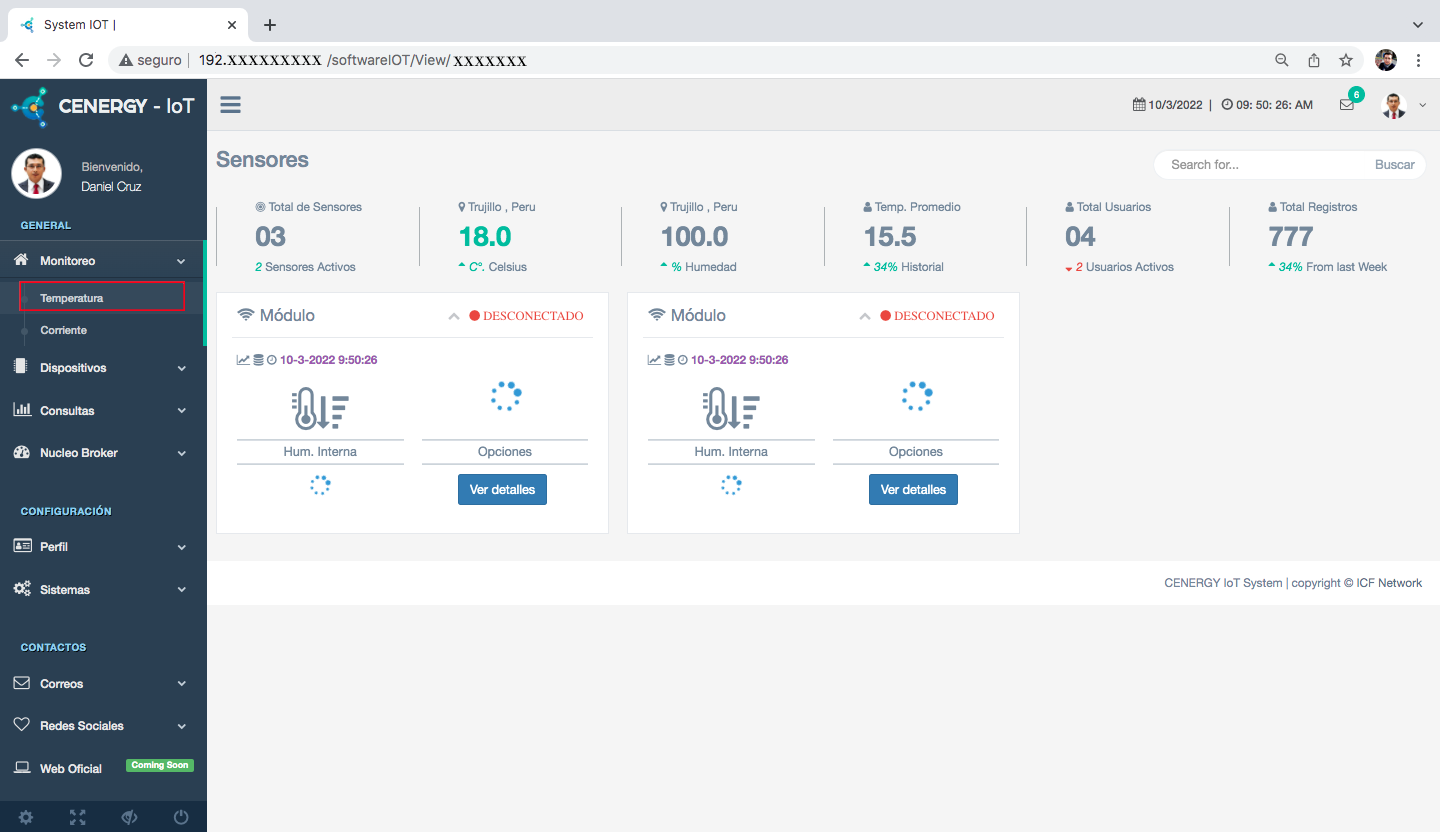
\includegraphics[width=1.55\textwidth]{./Figures/gui/2.png}
\caption{Interfaz gráfica de usuario donde se listan los sensores del sistema.}
\label{fig:gui2}
\end{figure}
\end{landscape} %

%%%%%%%%%%%%%%%%%%%%%%%%%%%%%%%%%%%%%%%%%%%%%%%%%%%

%%%%%%%%%%%%%%%%%%%%%%%%%%%%%%%%%%%%%%%%%%%%%%%%%%%
\begin{landscape} % esto es para rotar la pagina e imagen
\begin{figure}[htpb]
\centering 
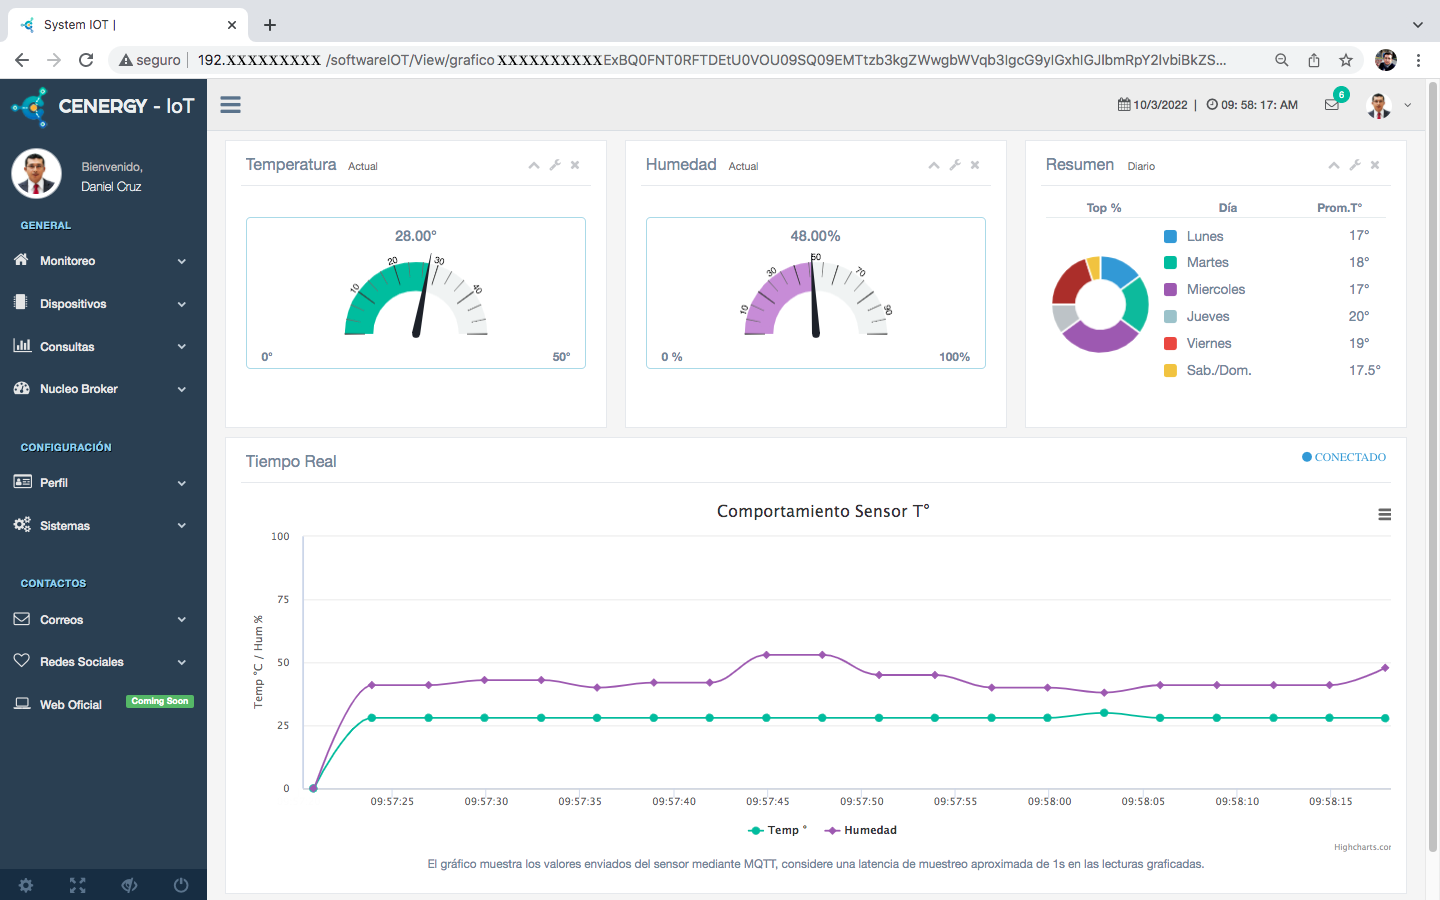
\includegraphics[width=1.5\textwidth]{./Figures/gui/2-1.png}
\caption{Interfaz gráfica de usuario donde se muestran todos los detalles de un sensor.}
\label{fig:gui2-1}
\end{figure}
\end{landscape} %

%%%%%%%%%%%%%%%%%%%%%%%%%%%%%%%%%%%%%%%%%%%%%%%%%%%

%%%%%%%%%%%%%%%%%%%%%%%%%%%%%%%%%%%%%%%%%%%%%%%%%%%
\begin{landscape} % esto es para rotar la pagina e imagen
\begin{figure}[htpb]
\centering 
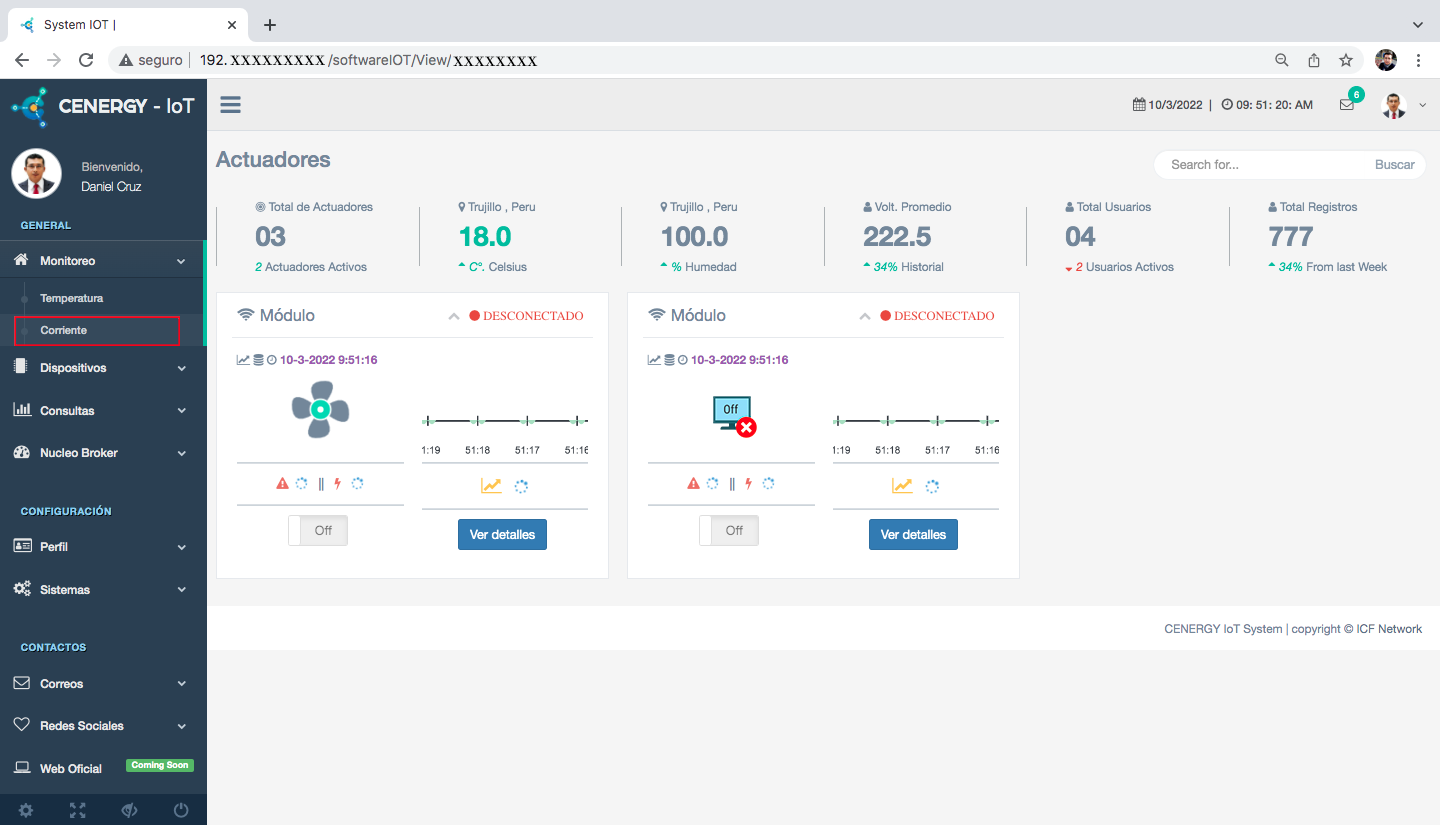
\includegraphics[width=1.52\textwidth]{./Figures/gui/3.png}
\caption{Interfaz gráfica de usuario donde se listan los sensores de consumo junto a su función de actuador.}
\label{fig:gui3}
\end{figure}
\end{landscape} %

%%%%%%%%%%%%%%%%%%%%%%%%%%%%%%%%%%%%%%%%%%%%%%%%%%%

%%%%%%%%%%%%%%%%%%%%%%%%%%%%%%%%%%%%%%%%%%%%%%%%%%%
\begin{landscape} % esto es para rotar la pagina e imagen
\begin{figure}[htpb]
\centering 
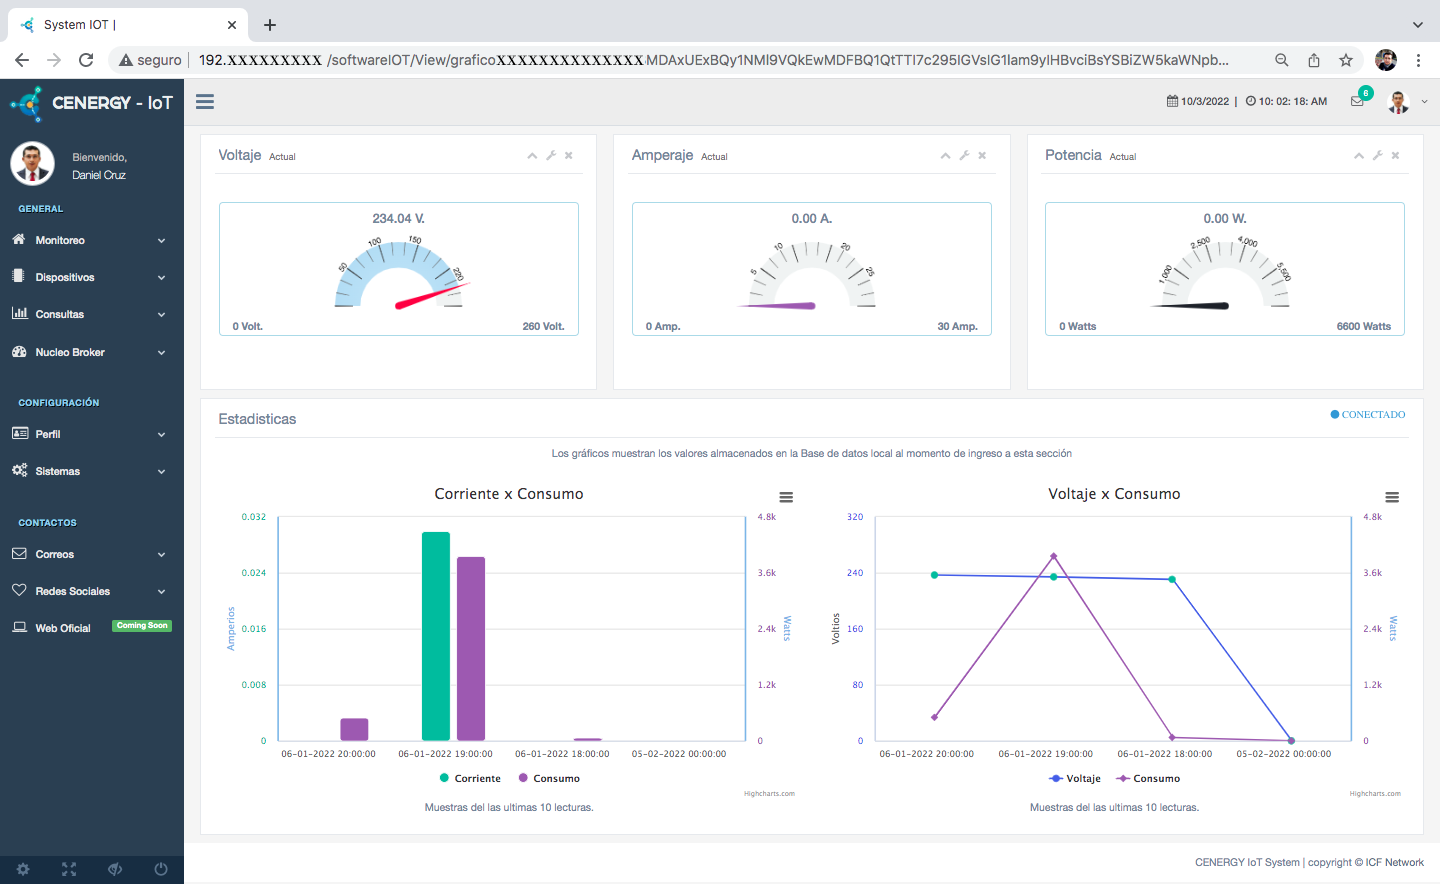
\includegraphics[width=1.52\textwidth]{./Figures/gui/3-1.png}
\caption{Interfaz gráfica de usuario donde se muestran todos los detalles de un sensor de consumo.}
\label{fig:gui3-1}
\end{figure}
\end{landscape} %

%%%%%%%%%%%%%%%%%%%%%%%%%%%%%%%%%%%%%%%%%%%%%%%%%%%

%%%%%%%%%%%%%%%%%%%%%%%%%%%%%%%%%%%%%%%%%%%%%%%%%%%
\begin{landscape} % esto es para rotar la pagina e imagen
\begin{figure}[htpb]
\centering 
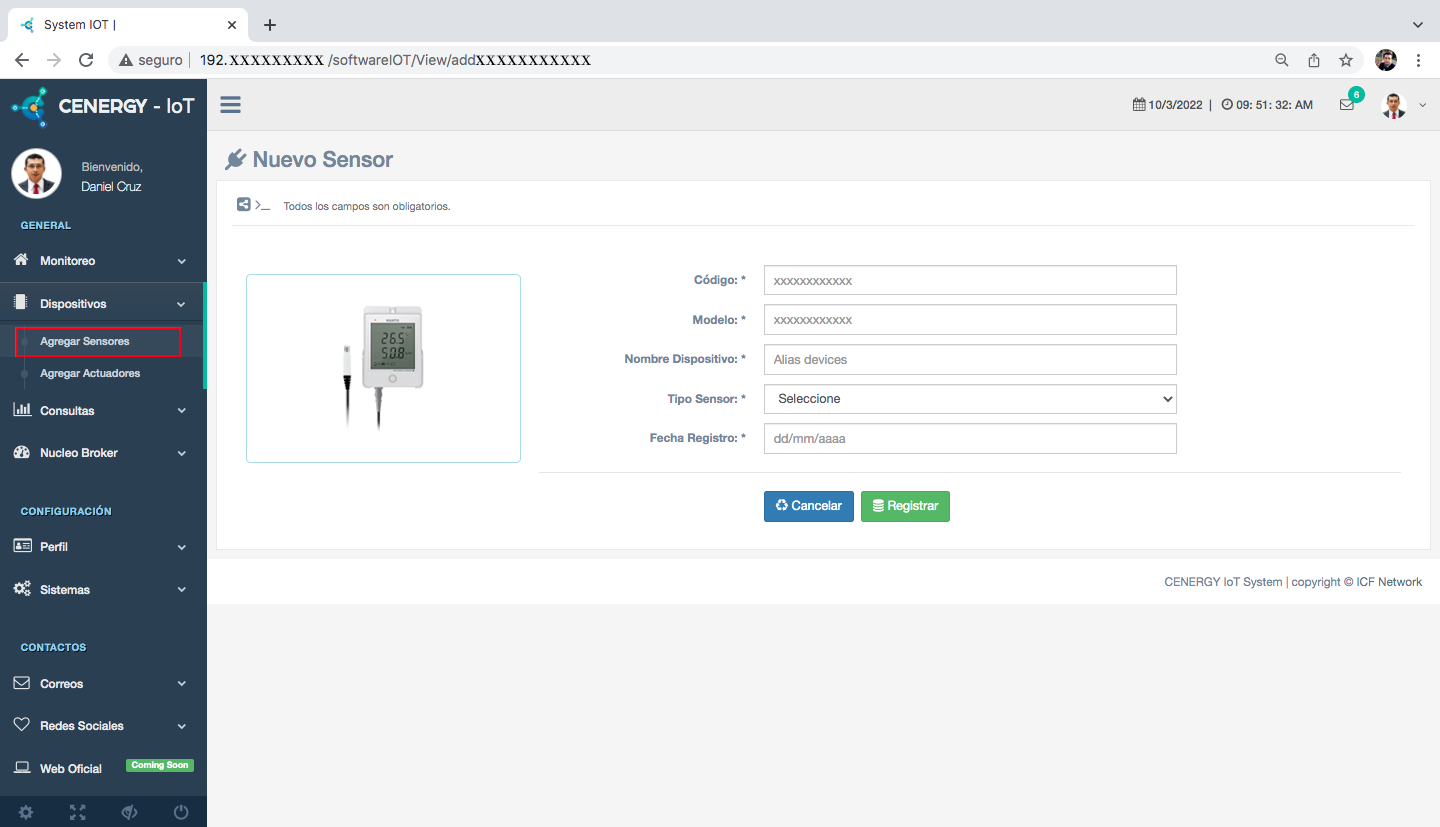
\includegraphics[width=1.55\textwidth]{./Figures/gui/4.png}
\caption{Interfaz gráfica de usuario para agregar un nuevo dispositivo al sistema.}
\label{fig:gui4}
\end{figure}
\end{landscape} %

%%%%%%%%%%%%%%%%%%%%%%%%%%%%%%%%%%%%%%%%%%%%%%%%%%%

%%%%%%%%%%%%%%%%%%%%%%%%%%%%%%%%%%%%%%%%%%%%%%%%%%%
\begin{landscape} % esto es para rotar la pagina e imagen
\begin{figure}[htpb]
\centering 
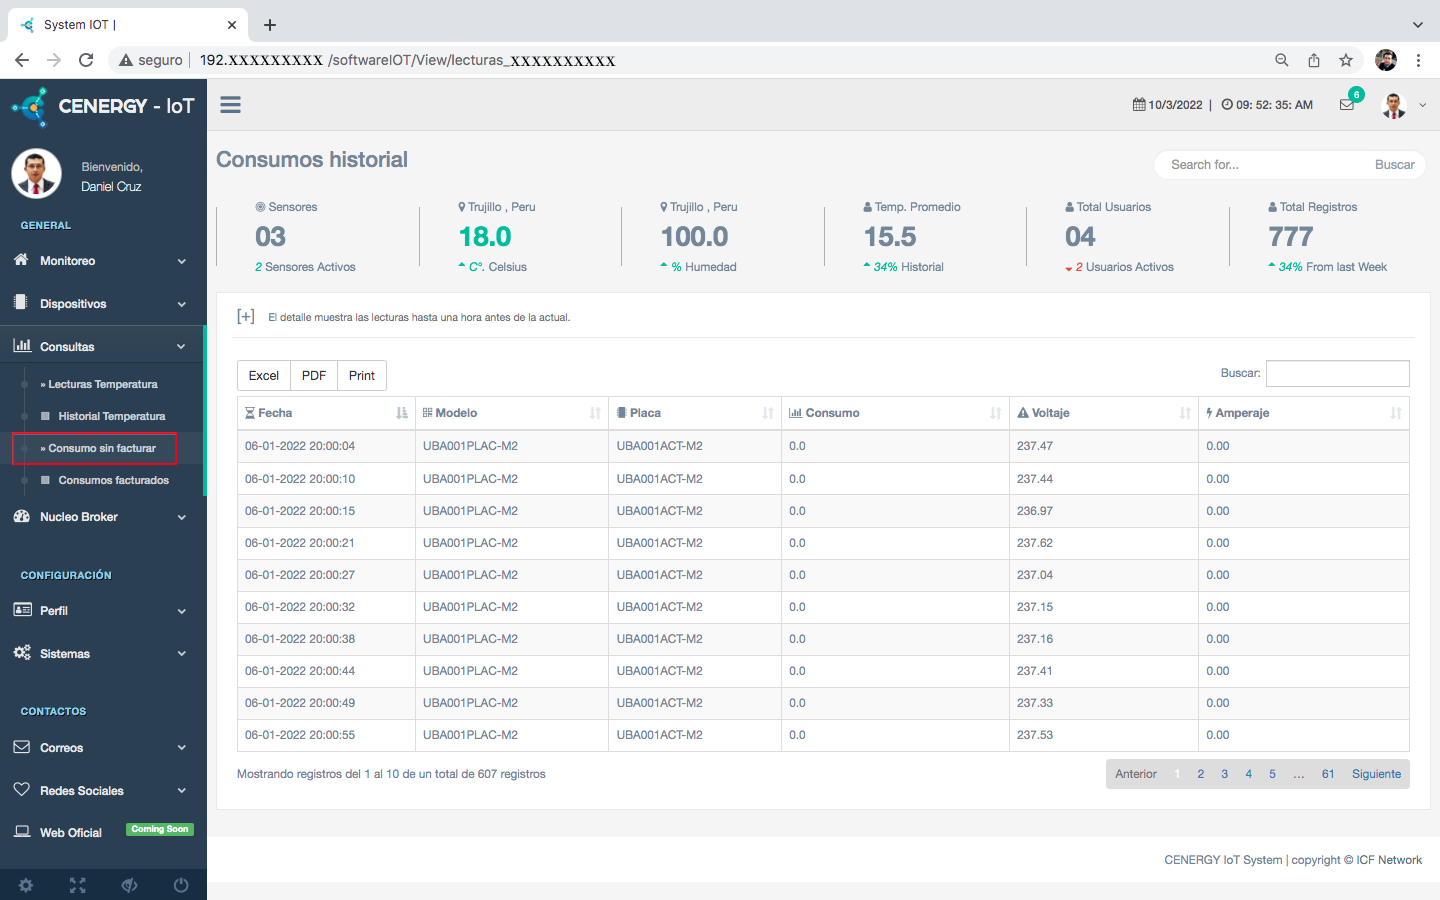
\includegraphics[width=1.5\textwidth]{./Figures/gui/5.png}
\caption{Interfaz gráfica de usuario donde se muestran las consultas y reportes de la base de datos.}
\label{fig:gui5}
\end{figure}
\end{landscape} %

%%%%%%%%%%%%%%%%%%%%%%%%%%%%%%%%%%%%%%%%%%%%%%%%%%%
\begin{landscape} % esto es para rotar la pagina e imagen
\begin{figure}[htpb]
\centering 
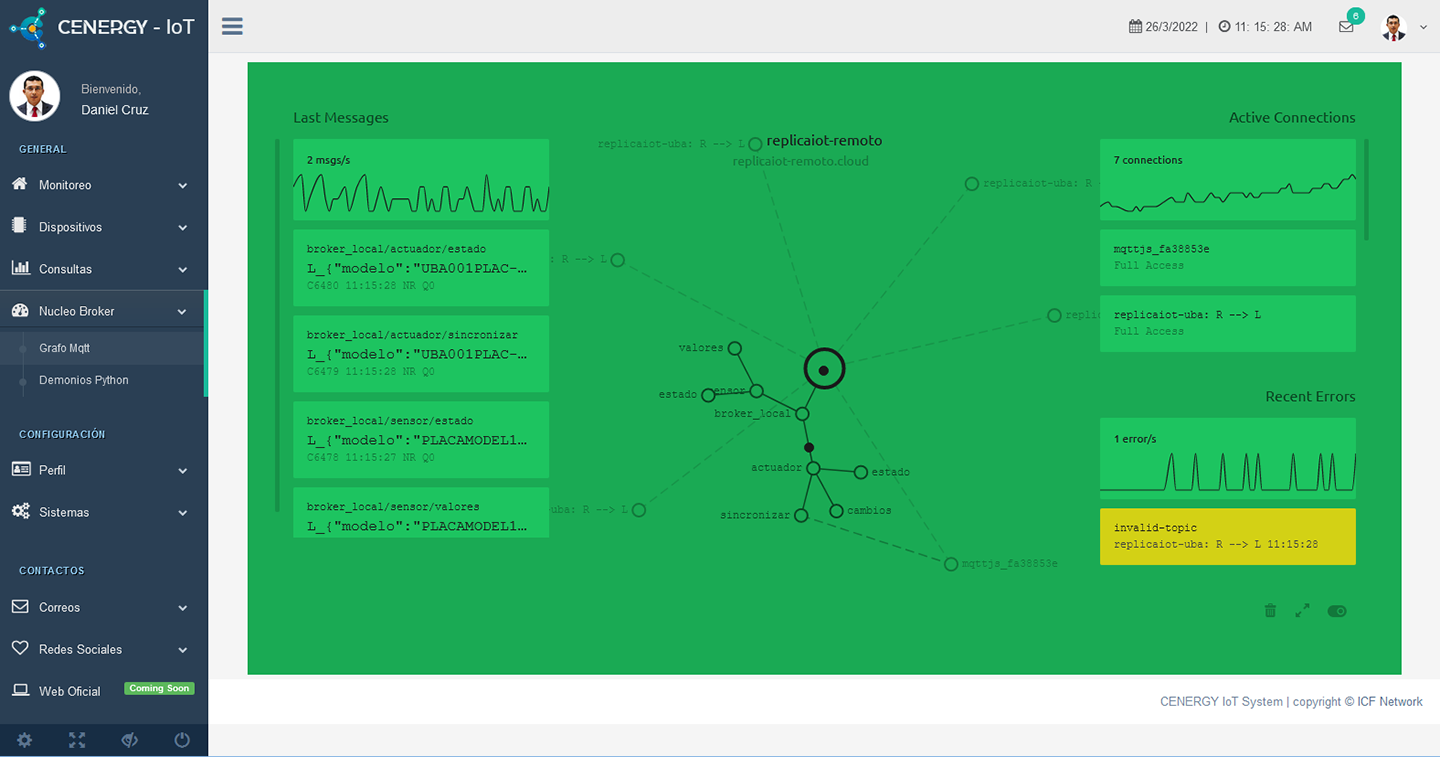
\includegraphics[width=1.5\textwidth]{./Figures/gui/nucleo.png}
\caption{Grafo de comunicación y sincronización del núcleo del sistema IoT.}
\label{fig:grafo}
\end{figure}
\end{landscape} %